\chapter{Implementation} \label{chap:implementation}
In this chapter, the implementation steps are introduced to the system described in
\ref{chap:system_design}. Two LIDAR sensors are placed on a simulated quadcopter in Gazebo,
that cover the top and bottom hemispheres around the drone. Using the data collected in the
simulator, these range measurements are filtered to simulate a number of VL53L1X sensors with
predefined operating modes and orientations.

In order to simulate the VL53L1X sensors accurately a set of parameters, capabilities, and
limitations of the LIDAR sensor is measured. Data is collected using selected operating modes
on selected distances that are described in \ref{sect:vl53l1x_measurements}. Average distance,
standard deviation, sampling rate, and typical range status are extracted.

The two main components in the evaluation of the VL53L1X sensor are a microcontroller and a PC. The
microcontroller communicates with the sensor and sends the raw measurements to the PC that runs
data processing and evaluates the received data. I chose to separate data collection and processing
because data processing is significantly easier in high-level programming languages like Python and
is much easier to adjust. It also enables data collection and offline processing.


\section{VL53L1X measurement setup}
For each measurement a combination of parameters needs to be configured on VL53L1X, these are the
timing budget, resolution, and distance preset. The configuration is done via the I2C protocol by the
microcontroller. VL53L1 API from STMicroelectronics is used for interfacing the sensor with the most
recent version at the time: 2.3.3. After completing boot the recommended initialization steps are
used, as described in example codes and the API user manual \cite{VL53L1XAPIManual}.

Each measurement is triggered in single-shot mode, which means exactly one ranging is done by the
sensor, and afterward, it waits until a new command arrives.  Single-shot is preferred over continuous
measurements because if the resolution is set to higher than 1x1, measurements need to be done on
multiple ROIs, and ROI has to be configured before triggering each measurement. In continuous mode,
the ROI cannot be modified between measurements.
A scan is complete if ranges are done on all ROIs of interest. The completed scan is then forwarded
for processing to the PC via USB-CDC protocol.

\begin{figure}[ht]
    \centering
    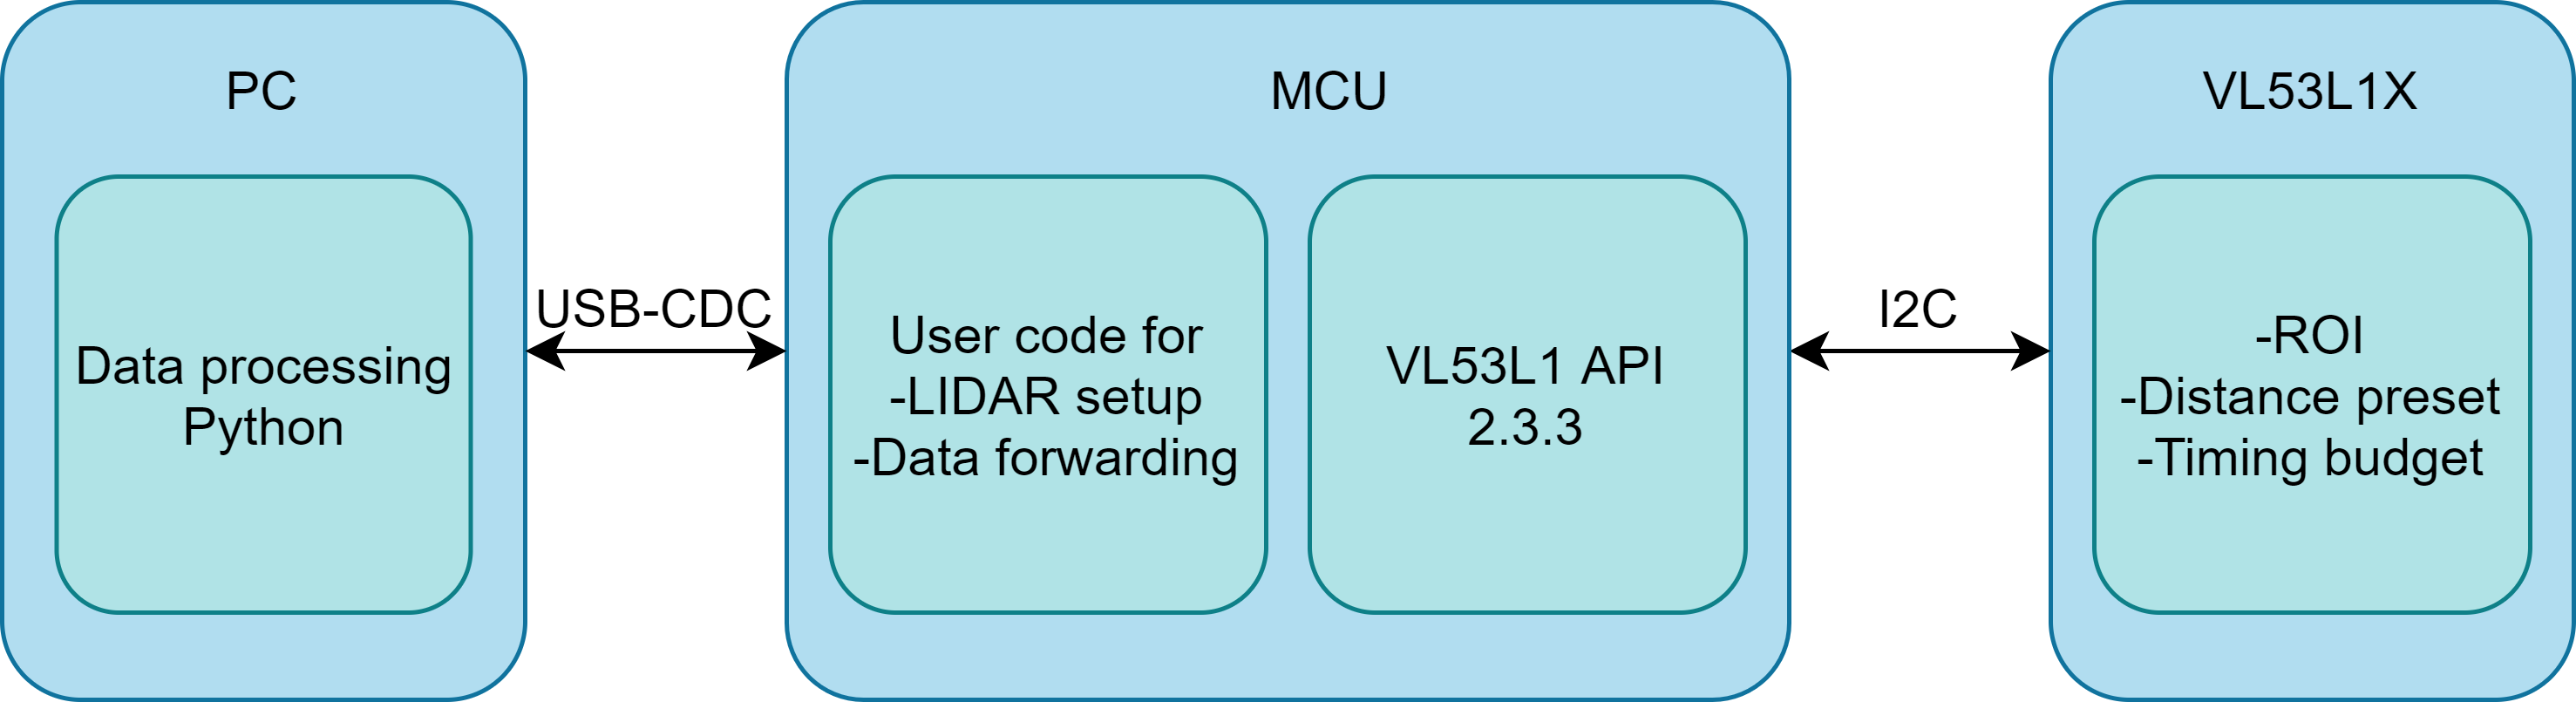
\includegraphics[width=130mm, keepaspectratio]{figures/vl53l1x_workflow.png}
    \caption{VL53L1X measurement workflow}
    \label{fig:vl53l1x_workflow}
\end{figure}


I chose Python as a programming language to read data from USB-CDC protocol and process the incoming
data because Python is rich in data processing tools and enables quick development. The script first
reads 50 scans coming from the MCU, then closes communication and works on the collected data.
The features extracted are the average distance, standard deviation, typical range status, and sampling
time. The average and standard deviation are calculated based on the whole population as in equations
\ref{eq:avg} and \ref{eq:std}, where s and r are the indices of scan and range, S and R are the
number of scans and ranges accordingly.

\begin{equation} \label{eq:avg}
    d_{avg}=\frac{1}{S \cdot R}\sum_{s=0}^S{\sum_{r=0}^R{d_{sr}} }
\end{equation}

\begin{equation} \label{eq:std}
    d_{std}=\sqrt{ \frac{1}{S\cdot R}\sum_{s=0}^S{ \sum_{r=0}^R{ (d_{sr} -d_{avg}})^2 }}
\end{equation}


\subsection{Comparison of selected operating modes}
VL53L1X LIDAR sensor has an adjustable timing budget from 18.5ms all the way to 1 second, which
determines the maximum time a ranging operation can take. To see the effect of the timing budget with
different ROI setups and distance modes, 4 timing budgets have been selected.

With an 18.5ms budget, the sensor operates on the highest possible measurement frequency of 50Hz. This
can only be achieved in short distance mode without the possibility of modifying the ROI. The second
selected budget is 33ms, which is the lowest possible value to be used with long-distance preset.
140ms is the lowest value that can provide measurements up to 4 meters. Lastly, the 200ms budget is
selected to see how a higher timing budget affects accuracy. It is also the value used in the
VL53L1X datasheet\cite{VL53L1XDatasheet} to demonstrate ranging accuracy.

The calculated average distance and standard deviation against the real distance can be seen on
figure \ref{fig:vl53l1x_meas_opmodes}, STD separately is on \ref{fig:vl53l1x_meas_opmodes_std}.
The measured sampling time accordingly is visible in figure \ref{fig:vl53l1x_meas_opmodes_sampling}.

Based on the completed measurements, it can be seen that sampling time is independent of the
distance preset in use and is directly proportional to the number of ROIs in a scan and the
timing budget. 50Hz sampling rate is not achieved even with an 18.5ms timing budget, because
the LIDAR was used in single-shot mode and each measurement needs to be triggered by the MCU.
Sampling time can be increased for setups with 1x1-resolutions by switching to continuous
measurement mode.

In every setup on each distance, the most accurate measurement is always with
resolution 1x1. By increasing the resolution, therefore lowering the receiver SPAD array size,
the measured distance starts to deviate from the real distance, and STD increases. This can be
seen at 2.5m distance with medium preset. Long-distance preset however produces more accurate
measurements even on 3m, so it is preferred over medium preset.

Measurements with long-distance preset and 140ms timing budget follow the real distances
even on 3 meters but start to deviate at 3.5 meters with 2x2-resolution and above. Raising
the timing budget to 200ms reduces the error and standard deviation, but doesn't eliminate
completely.


\begin{figure}[ht]
    \centering
    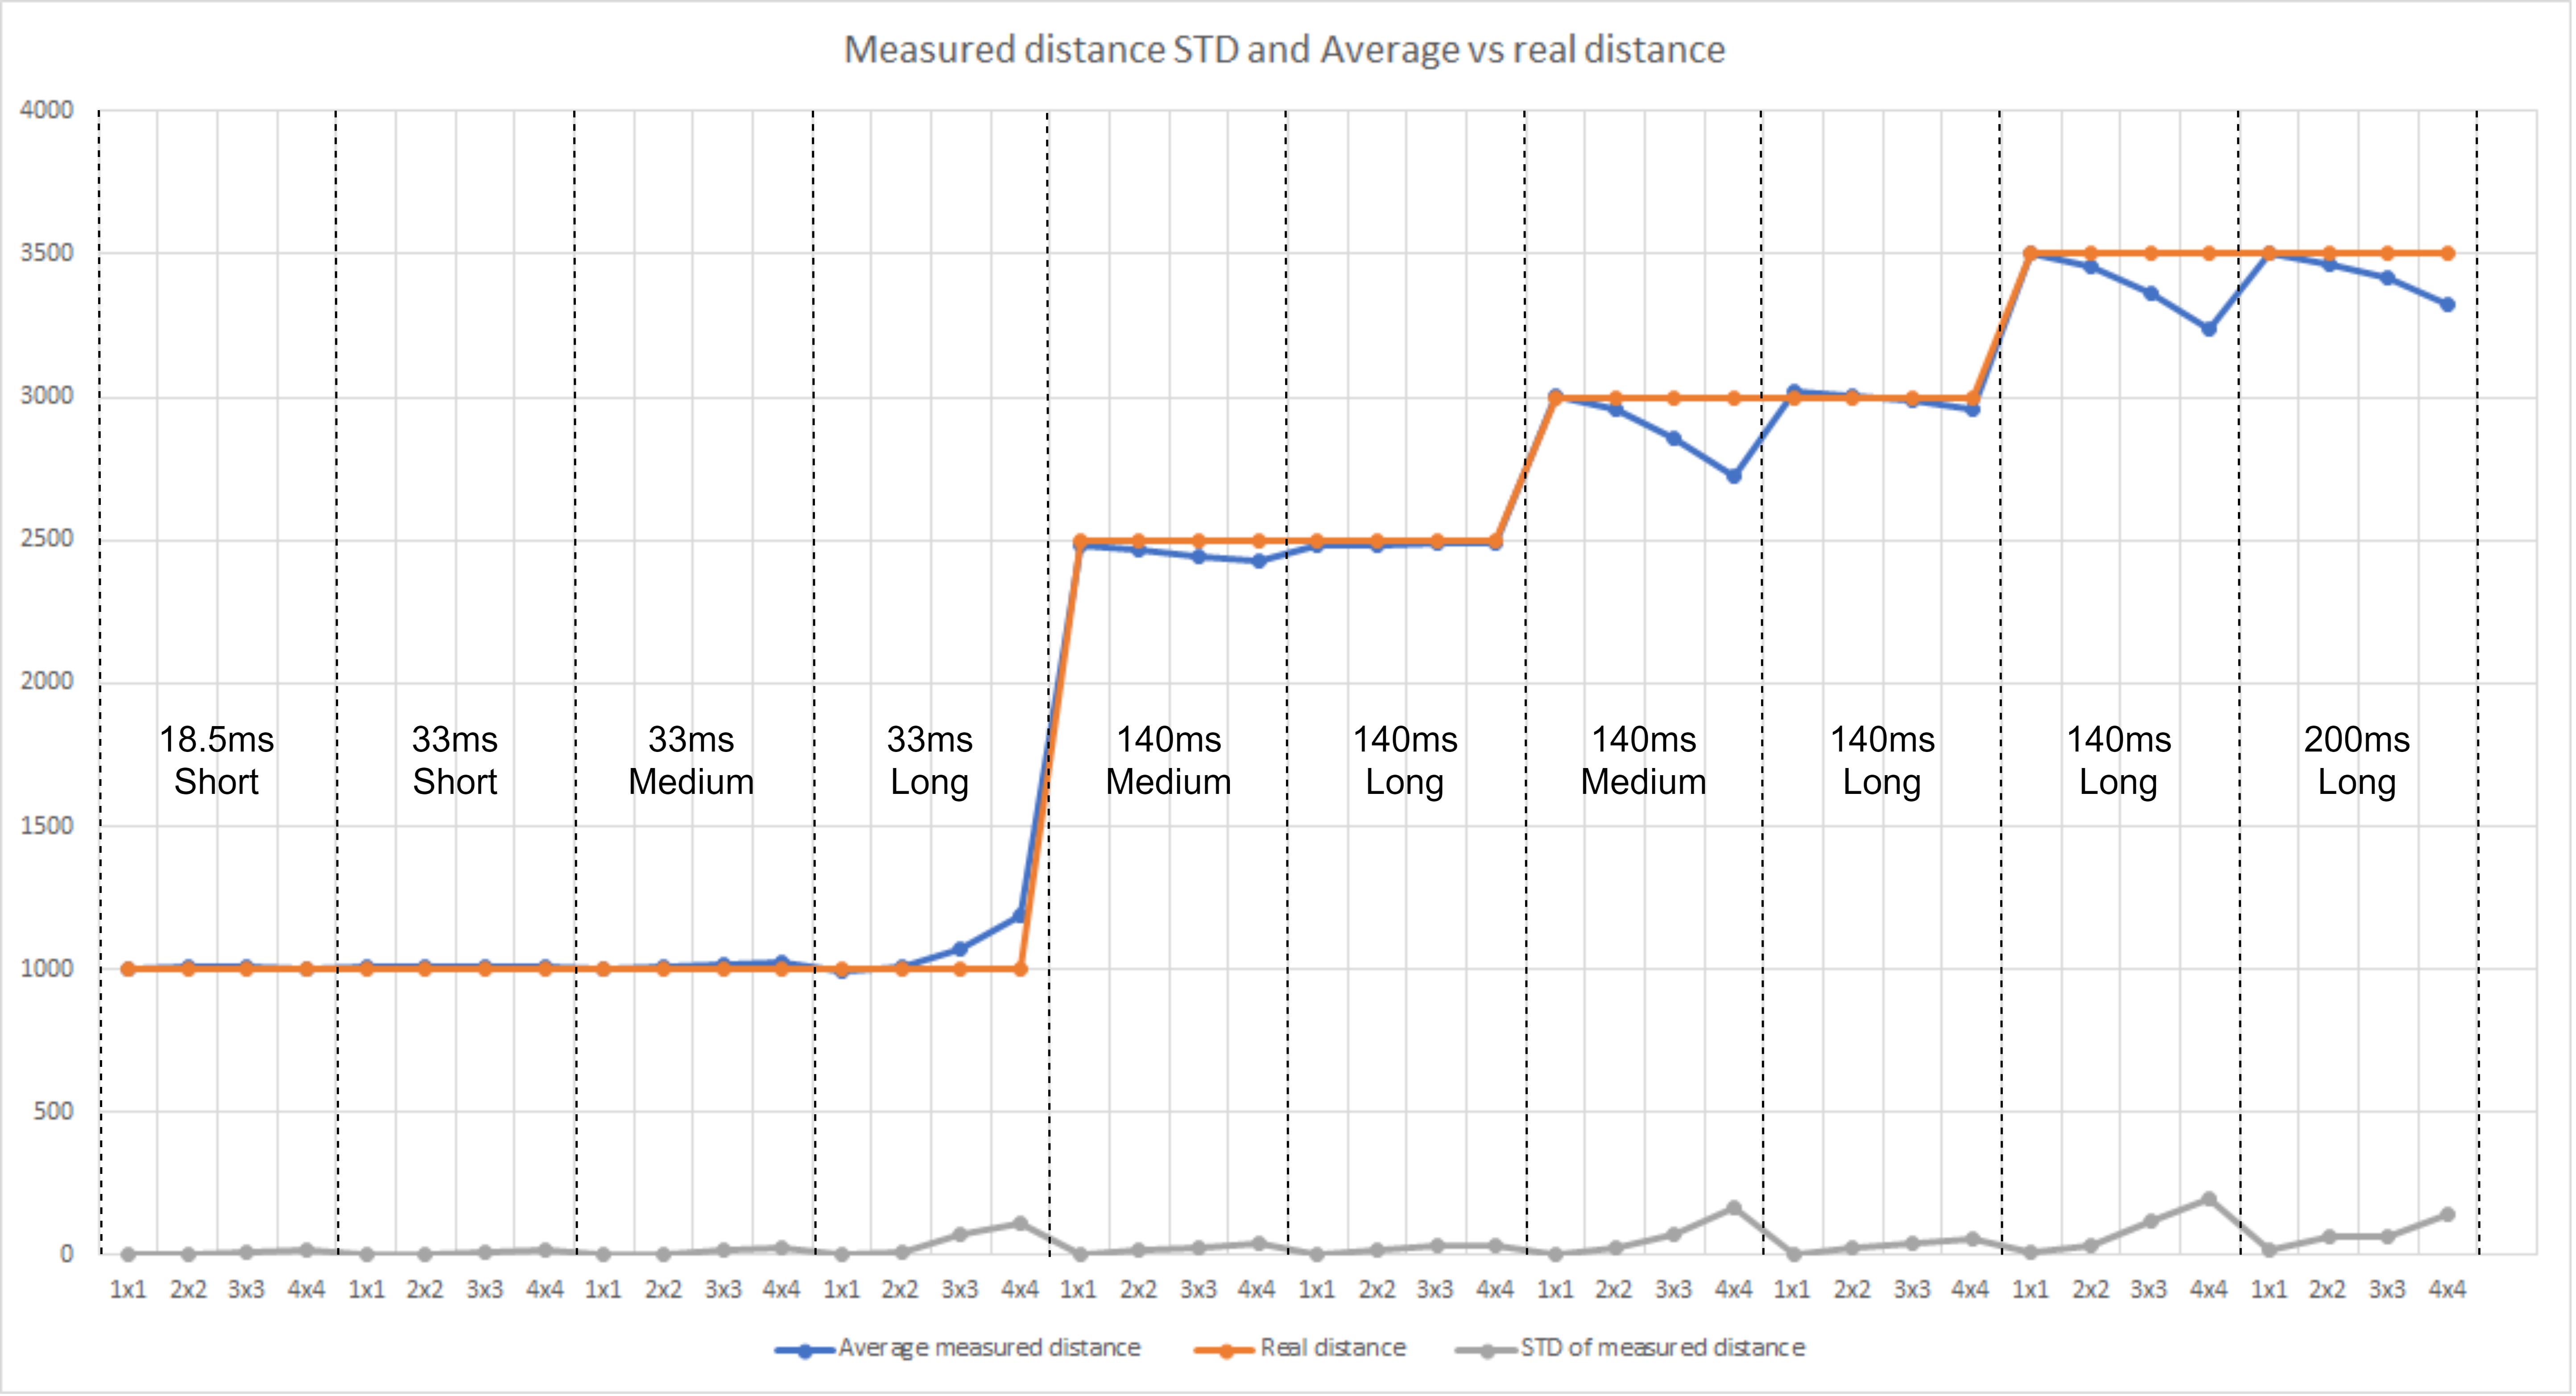
\includegraphics[width=150mm, keepaspectratio]{figures/vl53l1x_measurements_opmodes.png}
    \caption{VL53L1X measured distance STD and Average against real distance}
    \label{fig:vl53l1x_meas_opmodes}
\end{figure}
\begin{figure}[!h]
    \centering
    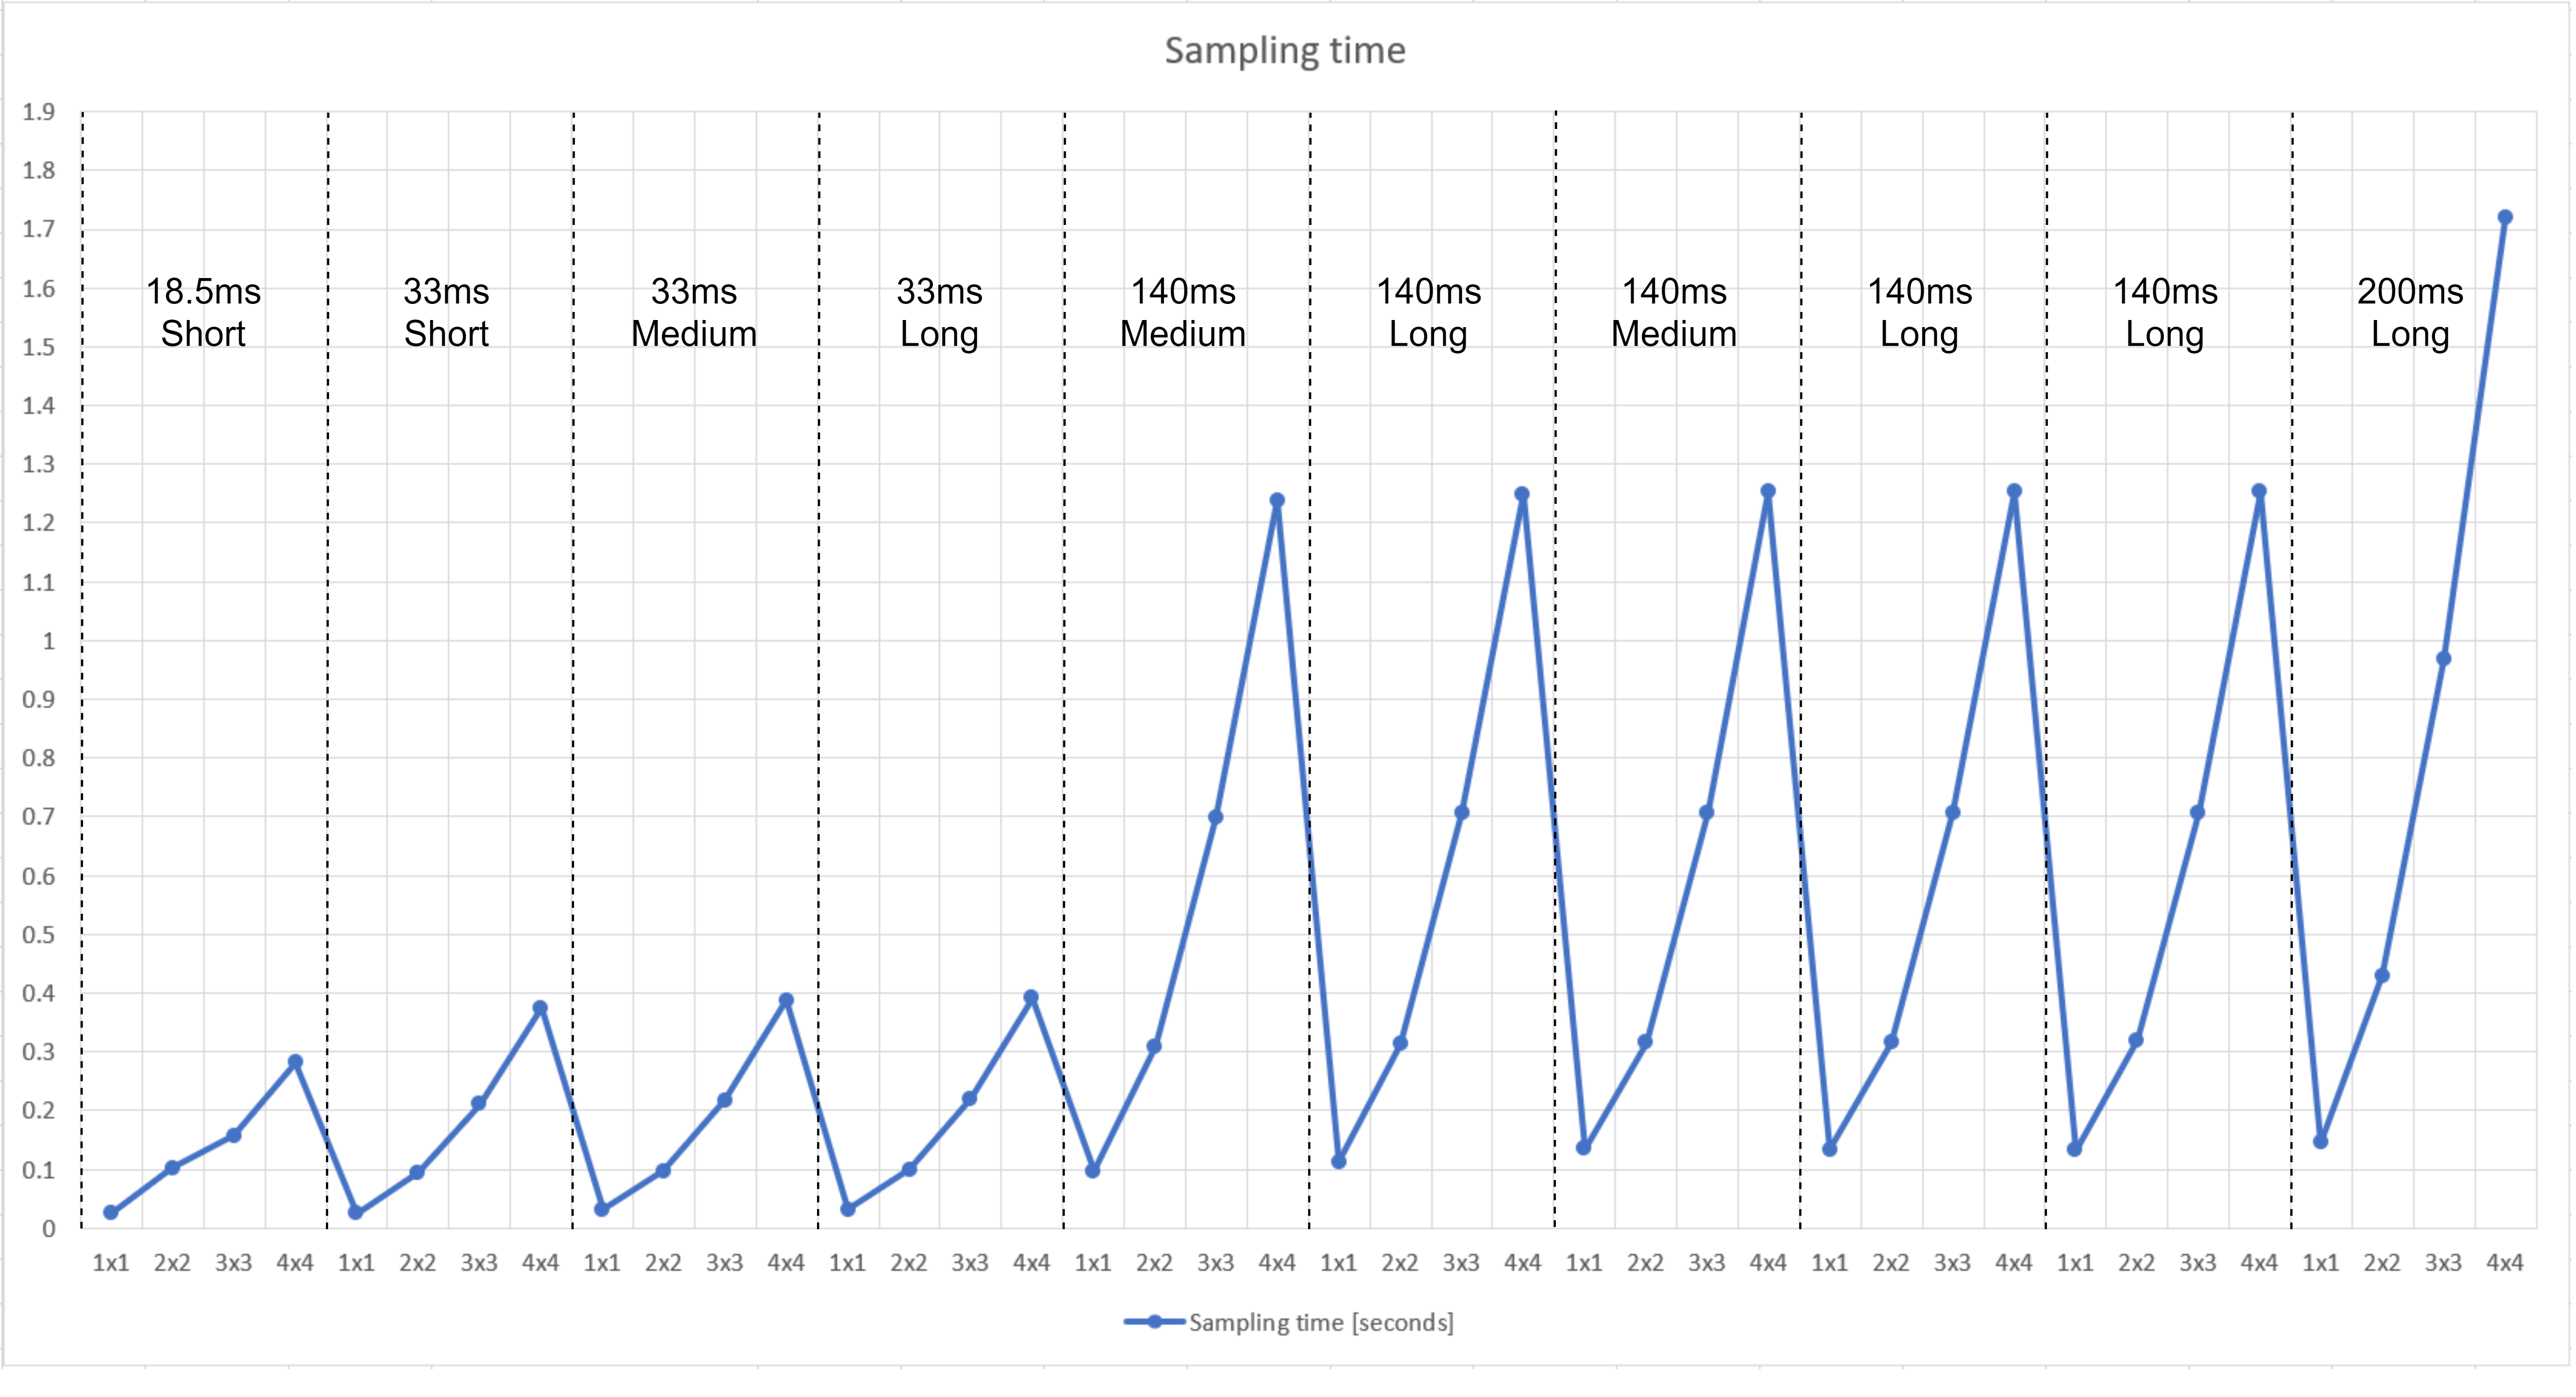
\includegraphics[width=150mm, keepaspectratio]{figures/vl53l1x_measurements_opmodes_sampling.png}
    \caption{VL53L1X range sampling time in different operation modes}
    \label{fig:vl53l1x_meas_opmodes_sampling}
\end{figure}

\newpage

\begin{figure}[!h]
    \centering
    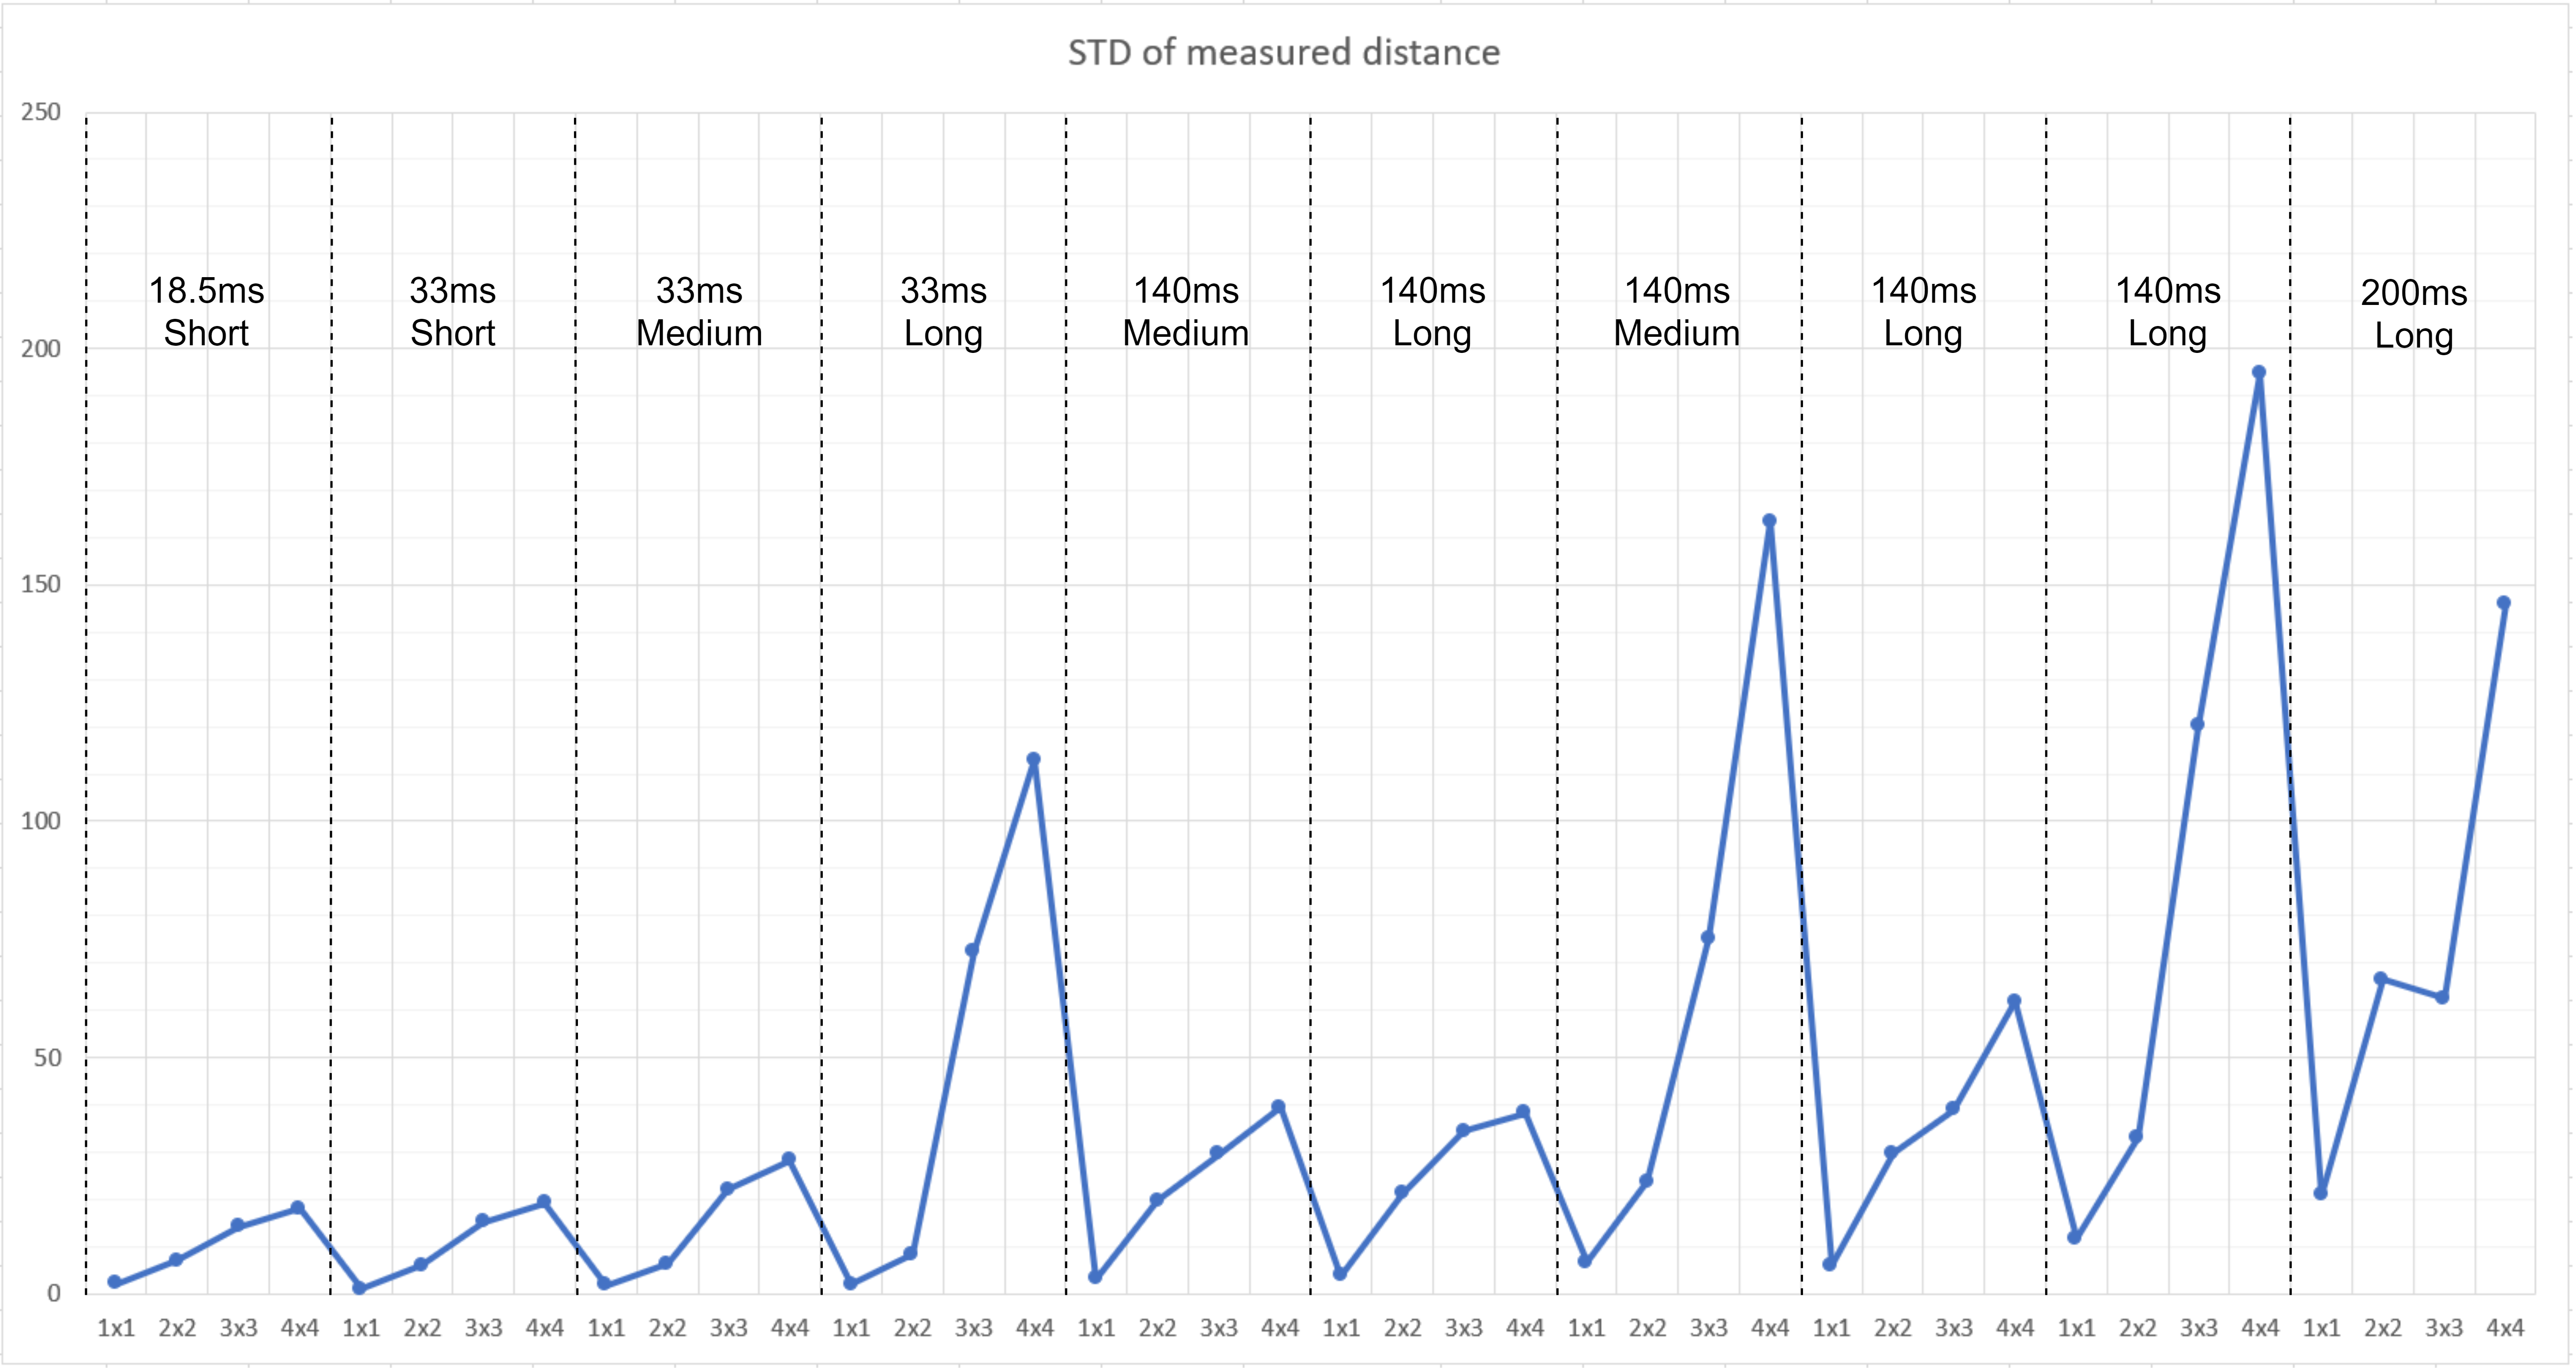
\includegraphics[width=150mm, keepaspectratio]{figures/vl53l1x_measurements_opmodes_std.png}
    \caption{VL53L1X standard deviation of ranges in different operation modes}
    \label{fig:vl53l1x_meas_opmodes_std}
\end{figure}

\subsection{Detailed distance measurements} \label{sect:vl53l1x_detailed_measurements}
Based on the measurements described in the previous section, I chose a small set of LIDAR settings
to further investigate and see how these behave on different distances. These settings are
candidates to be used in simulations. The goal with the setting selection is to choose the ones
that may have a greater effect on the SLAM performance.

After the initial tests with Cartographer SLAM, it's safe to assume that sampling time shouldn't be
greater than 500ms. This is not a strict threshold, but with higher sampling time, the algorithm
would have a hard time to follow the position of the drone and insert new scans precisely. The second
assumption is that more points per scan increase the performance of scan insertion because more points
create a more detailed and therefore more unique image.

I chose 5 setups for further investigation, 4 with each resolution and the fastest one with 18.5ms
timing budget. The lowest timing budget to be used with 4x4-resolution is 33ms, which is expected to be
just under the previously described threshold of 500ms per scan. The same budget is chosen for the 3x3-resolution,
while 2x2 has a lower number of ranges per scan so a higher budget, 70ms is selected to
have more accurate measurements. As for the 1x1-resolution, 18.5ms, and 140ms timing budgets are selected to see
the difference between a faster and a slower setup.

Each setup has been measured on distances starting from 0.5m to 4m with a step size
of 0.5m. The measurements can be seen in figures \ref{fig:vl53l1x_meas_detailed_dist},
\ref{fig:vl53l1x_meas_detailed_std}, \ref{fig:vl53l1x_meas_detailed_ts}. In the end,
all setups turned out to have a lower sampling time than 500ms. It is interesting, that
sampling time turned out to be higher on smaller distances and lower on high distances.
This might be because the internal algorithm of the VL53L1X sensor does longer measurements
to reassure that these ranges are not artifacts coming from reflections or crosstalk.

As expected the setup with 1x1-resolution and 140ms timing budget can range the farthest
with only 9mm standard deviation. The setup with 2x2-resolution deviates from the real
distance by 16cm on 3.5m but is still accurate at 3m.
The setups with 3x3- and 4x4-resolutions can measure up to 2.5m, but deviate on farther
measurements.

\begin{figure}[!h]
    \centering
	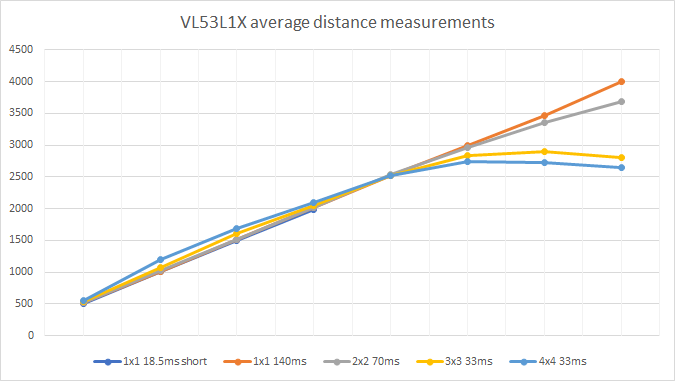
\includegraphics[width=115mm, keepaspectratio]{figures/vl53l1x_measurements_02_dist.png}
    \caption{Detailed distance measurements [mm]}
    \label{fig:vl53l1x_meas_detailed_dist}
\end{figure}

\begin{figure}[!h]
    \centering
	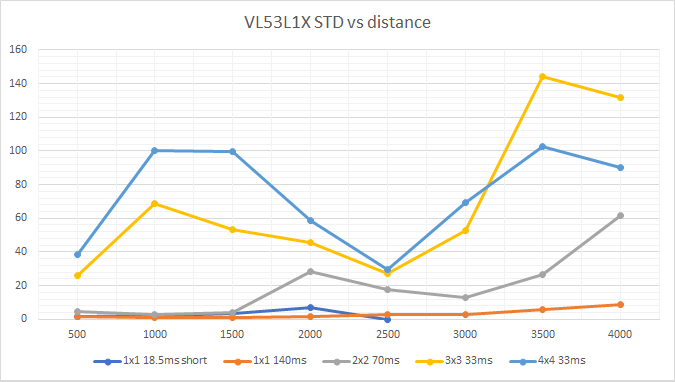
\includegraphics[width=115mm, keepaspectratio]{figures/vl53l1x_measurements_02_std.png}
    \caption{Standard deviation of selected measurements [mm]}
    \label{fig:vl53l1x_meas_detailed_std}
\end{figure}

\newpage

\begin{figure}[!h]
    \centering
	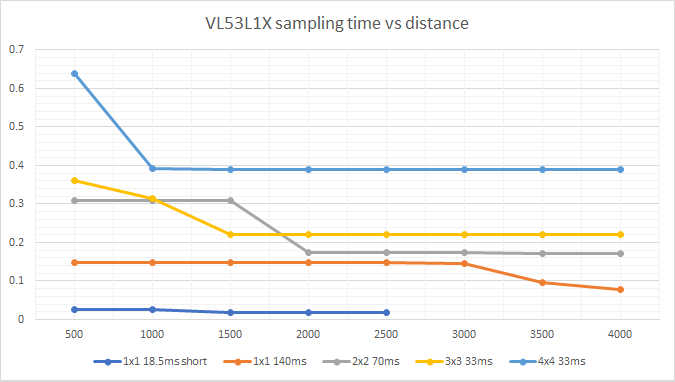
\includegraphics[width=115mm, keepaspectratio]{figures/vl53l1x_measurements_02_ts.png}
    \caption{Sampling time of selected measurements [s]}
    \label{fig:vl53l1x_meas_detailed_ts}
\end{figure}






\subsection{Detailed measurements with the fastest setup}
18.5ms timing budget with short distance preset can produce the fastest ranging measurements
up to 1.6m according to the datasheet. The short preset also has the best ambient light
immunity, a favorable quality. Due to these attributes, I have decided to do more measurements
using these settings in combination with all resolutions.

Surprisingly the sensor with these settings was able to measure up to 2m with 7mm
standard deviation only. Above 2m no ranges were successful, the sensor always reported 0 distance
instead.

In comparison to the previous results, the sampling time for each resolution has decreased
significantly. In the case of 4x4-resolution, the sampling time has decreased from 390ms to
265ms and the maximum distance from 2.5m to about 1m. The increase in the update rate might be
beneficial for the SLAM algorithm.

Surprisingly the update rate for 1x1-resolution reached 56Hz, which is higher than the
maximum update rate according to the datasheet. The reason for the increased update rate
is that 50Hz was calculated using continuous measurement mode that places a 1.5ms delay
between ranges. In this scenario, the device was used in single-shot mode and there was
no delay between measurements. Although this method puts a high load on the host
microcontroller that is not favorable in most applications.



\begin{figure}[!h]
    \centering
	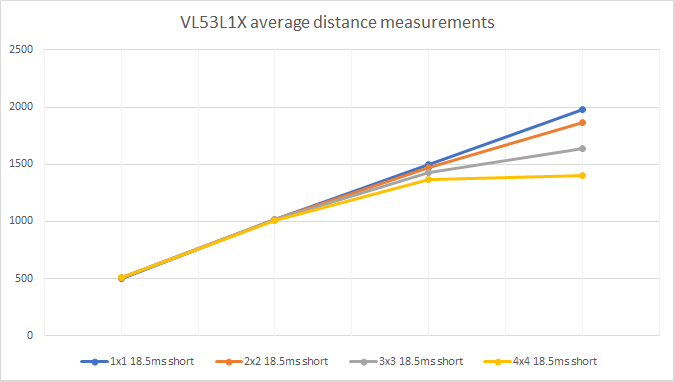
\includegraphics[width=115mm, keepaspectratio]{figures/vl53l1x_measurements_03_dist.png}
    \caption{Detailed distance measurements [mm]}
    \label{fig:vl53l1x_meas_further_detailed_dist}
\end{figure}

\begin{figure}[!h]
    \centering
	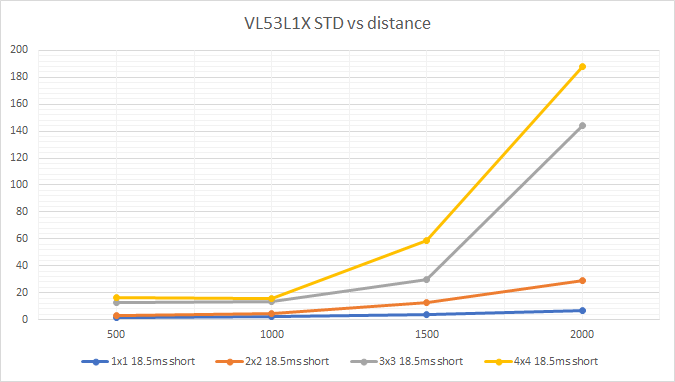
\includegraphics[width=115mm, keepaspectratio]{figures/vl53l1x_measurements_03_std.png}
    \caption{Standard deviation of selected measurements [mm]}
    \label{fig:vl53l1x_meas_further_detailed_std}
\end{figure}


\begin{figure}[!h]
    \centering
	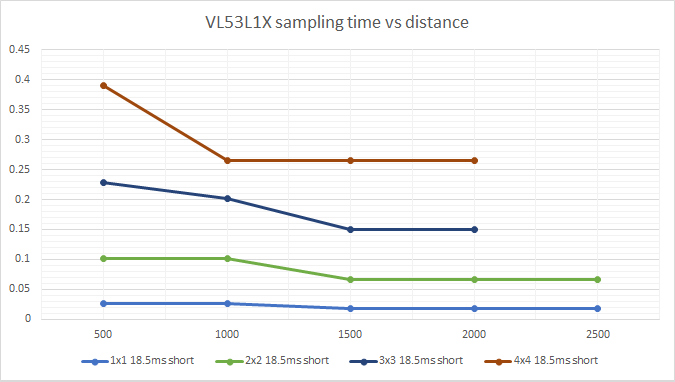
\includegraphics[width=115mm, keepaspectratio]{figures/vl53l1x_measurements_03_ts.png}
    \caption{Sampling time of selected measurements [s]}
    \label{fig:vl53l1x_meas_further_detailed_ts}
\end{figure}

\newpage








\section{2D SLAM evaluation}
During the evaluation both in 2D and 3D, the same collected data will be used. The length
of the collected Rosbag is 144 seconds and contains all messages coming from all nodes on all
topics. The LIDAR distance measurements are published on two PointCloud topics on 30Hz each
and IMU data is published by the PX4 flight controller stack on 50Hz.
The ground-truth pose data is extracted from the original dataset into a csv-file and will
be used for trajectory comparison in all scenarios. The original Rosbag is then filtered
to simulate a number of VL53L1X sensors with selected parameters. The filtered bags only
contain the converted PointCloud2 and IMU besides the necessary clock messages.

The evaluation of Cartographer SLAM happens in incremental steps. It's unclear what parameters
affect the performance the most, so instead of applying all of them at once, I chose to introduce
these LIDAR parameters incrementally one by one to see the effects of them independently
and work towards a complete set of parameters.

In the first simulation only converted but unfiltered range data is used, which has the
maximum possible sampling rate, 4m maximum distance, and 128x128-resolution in a total of
the top and bottom hemispheres. This will produce the most accurate map and localization
estimates, it is unlikely that any down-sampled dataset will produce better results.

As the second step the effect of the resolution is tested. 13 LIDAR sensors are placed
evenly on the horizontal axis and their resolution is set to 4x4 first and lowered to 3x3,
2x2 and 1x1. The sampling rate and maximum distance parameters are left unchanged.

To investigate the effect of the sampling rate, the resolution with the best performance
from the previous step is used, but with the sampling rate of the actual sensor. Finally,
the maximum distance is lowered, while keeping the same layout of the sensors.

After introducing all parameters, the number of sensors is lowered until the lowest number
is found, which is still capable of producing a decent quality map.







\newpage



\subsection{Effects of LIDAR resolution}
\subsubsection{Unfiltered data}
In this step, the range measurements inside the collected Rosbag are converted to PointCloud2
without filtering and get written to a new bag. The LIDAR ranges visualized in
Rviz can be seen in figure \ref{fig:01_maxed_lidar} to demonstrate the scan resolution.

\begin{figure}[!h]
    \centering
	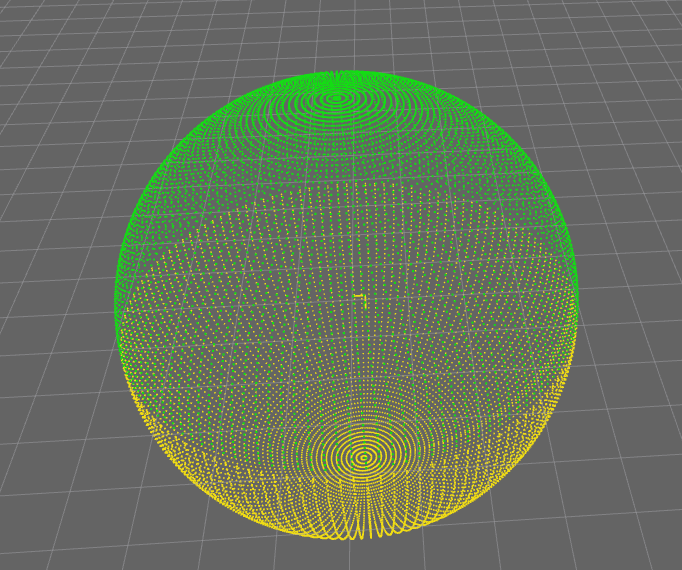
\includegraphics[width=70mm, keepaspectratio]{figures/01_maxed_lidar.png}
    \caption{Visualization of unfiltered LIDAR measurements maximized on 4 meters}
    \label{fig:01_maxed_lidar}
\end{figure}

Cartographer in 2D mode projects all points inside a scan to the horizontal plane before
insertion and therefore it is not advisable to include points that are coming from ranges
that are hitting the floor or the ceiling. Only points that are coming from reflections
of objects should be included in the scans and saturated LIDAR measurements should be
discarded. During the bandwidth filter step, Cartographer filters the points and only
inserts the ones inside user-set thresholds, others are discarded.

To exclude points coming from unwanted elevations or saturation, 4 parameters are
adjusted in the configuration file: min\_z, max\_z to set the interval on the z-axis
and min\_range, max\_range to set the range length interval. I have set min\_z and
max\_z values to -10cm and 50cm, min\_range and max\_range to 40cm and 370cm accordingly.
These settings proved to be working as expected and inserted ranges of the walls of
the building. Since scans of the whole sphere are published on two topics, these need to be
assembled into a single point cloud. This is done by Cartographer and is enabled by
setting num\_accumulated\_range\_data to 2.

IMU usage is enabled using the use\_imu\_data parameter and IMU data will be used as an
initial guess for the pose of the scan for insertion. Cartographer samples the
accelerometer values for a certain period of time to determine the direction of gravity.
The quadcopter changes pitch and roll angles quickly, so imu\_gravity\_time\_constant is
set to 0.5 seconds to enable the algorithm to follow quick movements.

After setting up the basic settings for interfacing Cartographer, the actual tuning of
the SLAM algorithm can be started. First, the submap size needs to be determined, which
depends on the sampling rate of the LIDAR sensor. It is important because a new submap
is built using constraints against the last two inserted submaps.
Setting submap size low will cause submaps to drift
or inadequate rotation due to the lack of reference points. On the other hand, setting submap
size high doesn't allow global SLAM thread to rearrange submaps and calculate loop closures
effectively.

\begin{figure}[!h]
    \centering
	$\vcenter{\hbox{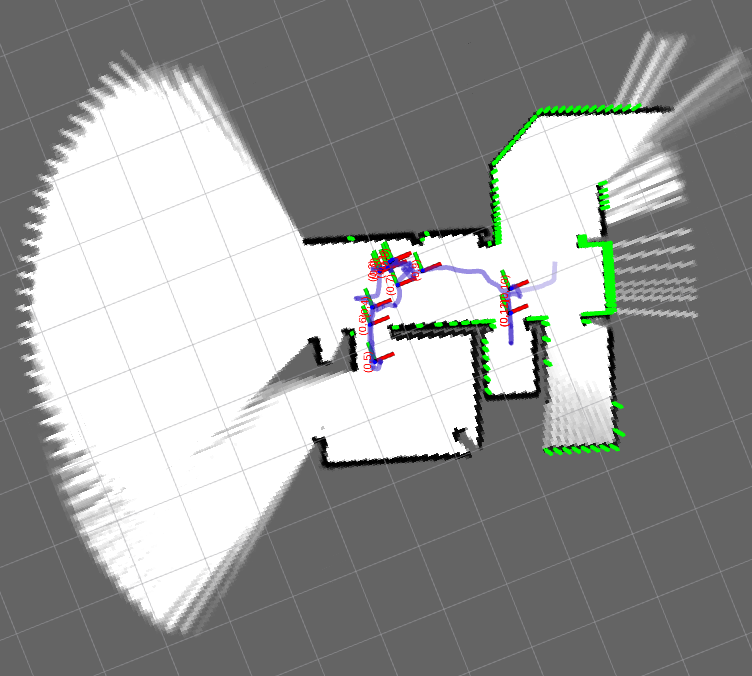
\includegraphics[height=60mm, keepaspectratio]{figures/01_SLAM_process_1.png}}}$
    $\vcenter{\hbox{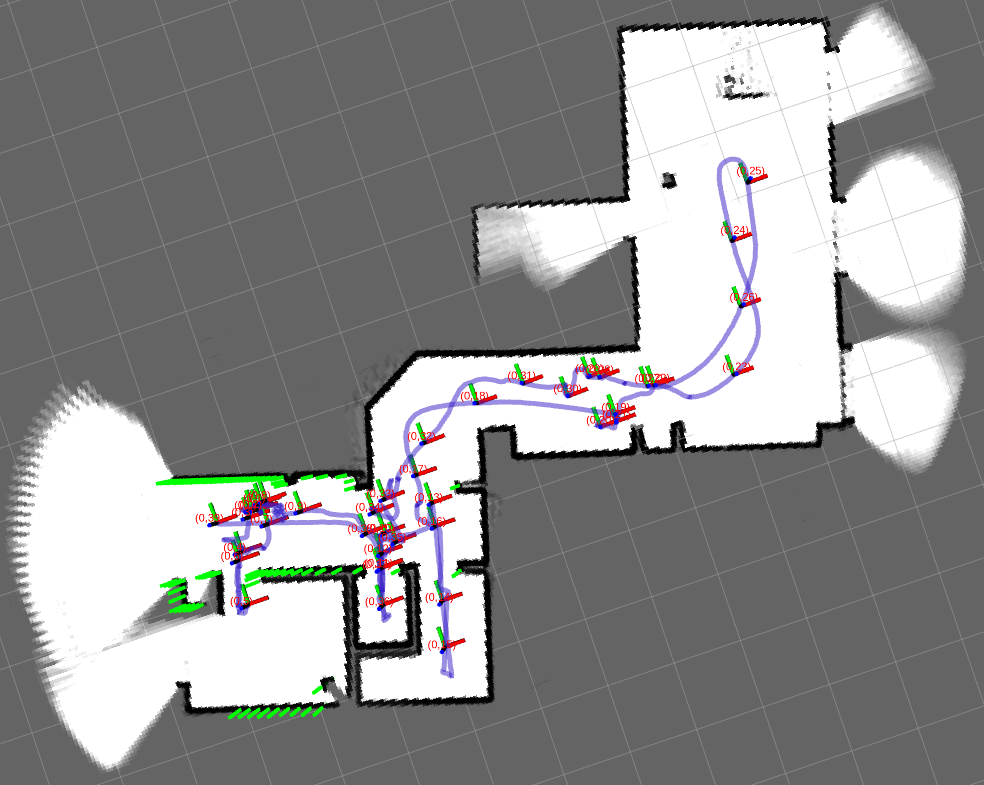
\includegraphics[height=60mm, keepaspectratio]{figures/01_SLAM_process_2.png}}}$
    \caption{2D SLAM map building on the left and complete map on the right}
    \label{fig:01_2d_slam_mapping}
\end{figure}

For tuning local SLAM, global SLAM is disabled. In this case, I found that lowering
translation\_weight and rotation\_weight under ceres scan matcher options increase the
mapping quality. The submap size is set to 90 ranges, which is too dense, but
due to the high sampling frequency and resolution, it still created an adequate map
as seen in figure \ref{fig:01_2d_slam_mapping}. Empty spaces are white color and
inserted scans are black. The green points on the visualization are the points
from the last inserted scan and the small coordinate systems are at the pose where
a submap has been completed.

Corners are sharp, walls are straight and even small details like columns are visible
on the final map. The big room on the top right of the map has three big windows and the drone
was flying about in the height of them and that's the reason for the high quantity of
empty space around this area. The algorithm was unable to insert points of the walls
between windows.

Because there is no noise added to ranges, even without global SLAM, a decent quality
map can be built. If global SLAM is enabled, the linear\_search\_window parameter needs
to be set to small, because the amount of drift of submaps is low. I have set the search
window to 25cm, so submaps cannot be moved further than 25cm. If it is left unchanged,
submaps in a range of 15 meters can be pulled together and would mess up the map.

\begin{figure}[!h]
    \centering
	$\vcenter{\hbox{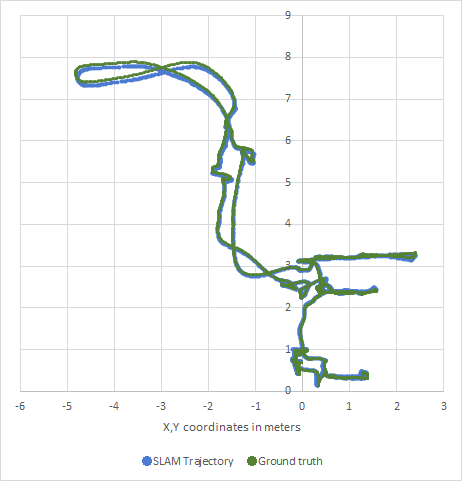
\includegraphics[height=65mm, keepaspectratio]{figures/01_trajectory.png}}}$
    $\vcenter{\hbox{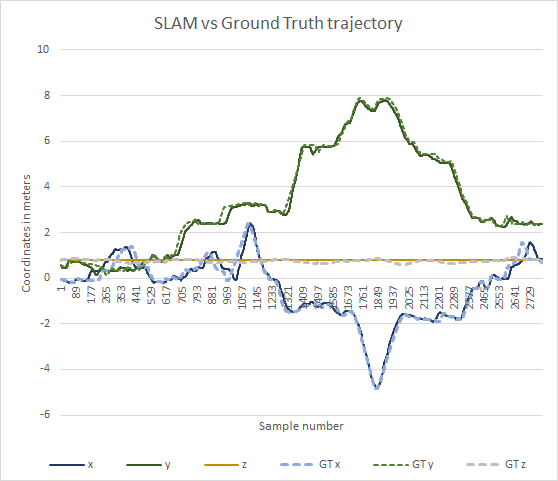
\includegraphics[height=65mm, keepaspectratio]{figures/01_trajectory_coordinates.png}}}$
    \caption{2D SLAM extracted trajectory against ground truth}
    \label{fig:01_trajectory}
\end{figure}

The extracted trajectory closely follows the ground truth trajectory as seen in figure
\ref{fig:01_trajectory}. The RMS error on the x- is 6.3cm and a bit less 6.5cm on the y-axis,
resulting in a cumulated 12.8cm RMS error.

\begin{figure}[!h]
    \centering
	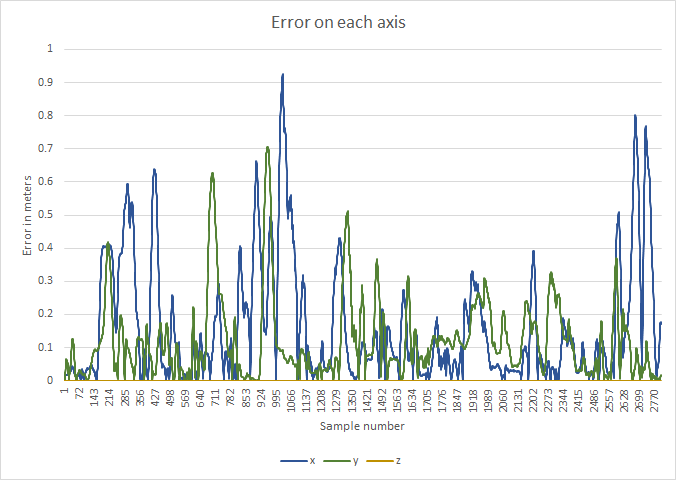
\includegraphics[height=65mm, keepaspectratio]{figures/01_trajectory_error.png}
    \caption{Trajectory error on each axis}
    \label{fig:01_trajectory_error}
\end{figure}

Figure \ref{fig:01_trajectory_error} shows the absolute error on the axes separately. The error
never goes above 25 centimeters on either axis and the fact that it always returns to 0 shows,
that there is no drift in the pose estimation. It can also be seen in figure
\ref{fig:01_trajectory}. Estimated and ground-truth coordinates overlap and produce a nicely
overlapping trajectory as on the left image.








\subsubsection{2D SLAM with 4x4-resolution}
In this scenario, the original Rosbag is filtered to simulate 13 LIDAR sensors placed
evenly on the horizontal axis as described in \ref{sect:lidar_layout_plan}, each with
4x4-resolution. The visualization of the point cloud from a single scan can be seen in
figure \ref{fig:02_lidar_layout}.

\begin{figure}[!h]
    \centering
	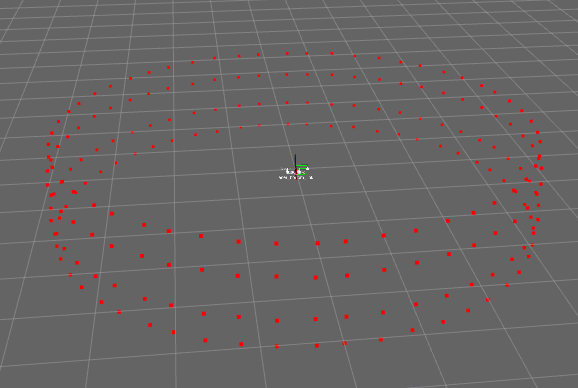
\includegraphics[height=50mm, keepaspectratio]{figures/02_lidar_layout.png}
    \caption{Visualization of ranges from 13 sensors with 4x4-resolution}
    \label{fig:02_lidar_layout}
\end{figure}

The tuning of the SLAM algorithm with this setup wasn't more difficult, than it was with
the previous setup, due to the high sampling rate and the high number of points in each scan.
For the local SLAM, I have set the translation\_weight to 8 and rotation\_weight to 15. The
reason for the increased weight is that otherwise the scan matcher algorithm was easily
moving and rotating scans to unreasonable positions. With the higher weights, the initial
guess of the pose has higher influence.

To simulate the behavior of VL53L1X, ranges inside the sensor's field of view are averaged.
This causes artifacts like curved corners and transition points that occur when an object is
only partly in the field of view and another distant object covers the rest of the view. These
smooth transitions hide the sharp edges of walls, making it harder to insert points and to
find loop-closures.

\begin{figure}[!h]
    \centering
	$\vcenter{\hbox{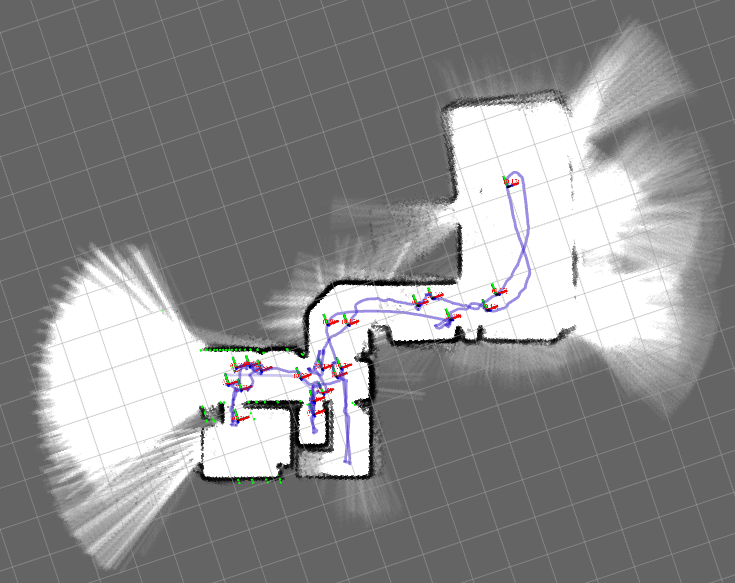
\includegraphics[height=55mm, keepaspectratio]{figures/02_before_loop_closure.png}}}$
    $\vcenter{\hbox{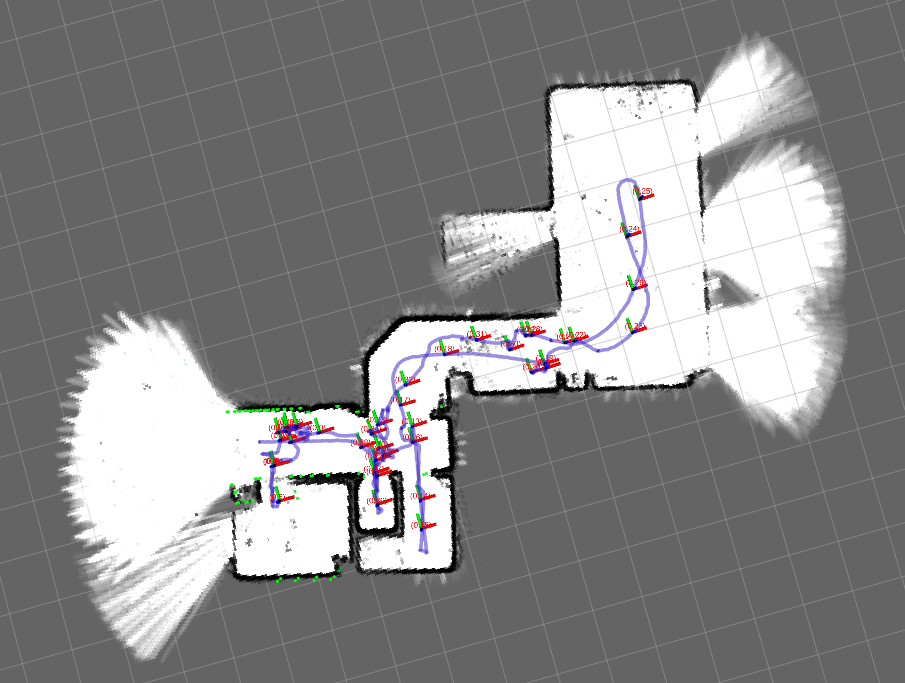
\includegraphics[height=55mm, keepaspectratio]{figures/02_after_loop_closure.png}}}$
    \caption{Map before and after tuning using 4x4-resolution}
    \label{fig:02_map}
\end{figure}

The final map after tuning is as seen in figure \ref{fig:02_map}. The left image shows the built
map before tuning and a failed loop-closure is seen in the top right of the map. The map on the
right at first glance is accurate, there are no major drifts in either rotation or placement.
Due to the averaging of the field of view, corners are curved and the walls are not as sharp as
they were using the unfiltered data. Transition points are best visible in the small room
that opens from the big room. These are caused by the drone flying by the door and a part of
a sensor's field of view hits the doorpost and the rest hits the wall behind. These ranges
are averaged to a single point in between the two objects. These points are always present
when the drone approaches a corner.

\begin{figure}[!h]
    \centering
	$\vcenter{\hbox{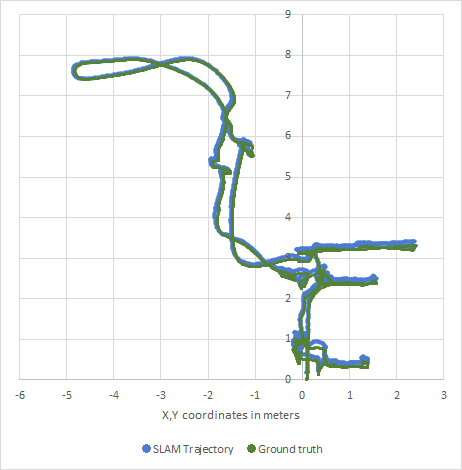
\includegraphics[height=65mm, keepaspectratio]{figures/02_trajectory.png}}}$
    $\vcenter{\hbox{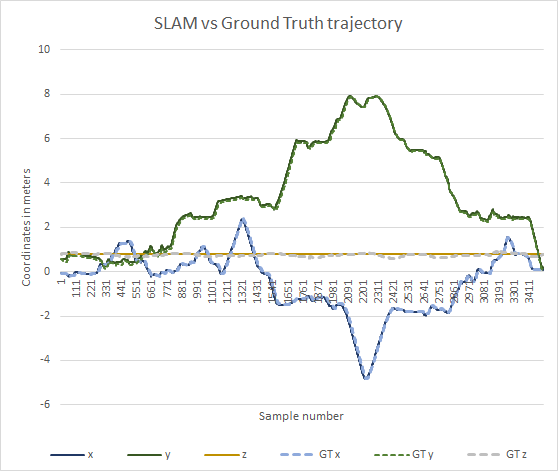
\includegraphics[height=65mm, keepaspectratio]{figures/02_trajectory_coordinates.png}}}$
    \caption{2D SLAM extracted trajectory against ground truth using 4x4-resolution sensors}
    \label{fig:02_trajectory}
\end{figure}

The estimated trajectory follows accurately the ground-truth trajectory as seen in
\ref{fig:02_trajectory}. As seen in the left picture, there is an offset between the two paths
and seems like a constant offset, but as seen in figure \ref{fig:02_trajectory_error}, there is
no constant offset on neither axes.

The RMS error of this setup is only 6cm more than the error of unfiltered data. The RMS error is 8.12cm
on the x- and 10.48cm on the y-axis, resulting in a cumulated error of 18.6cm.

\begin{figure}[!h]
    \centering
	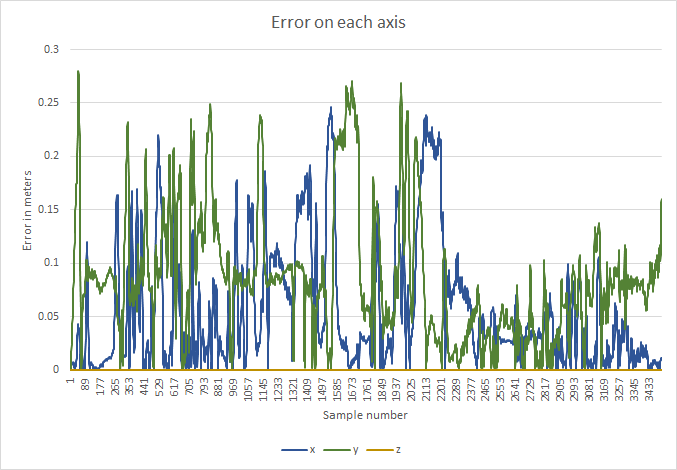
\includegraphics[height=65mm, keepaspectratio]{figures/02_trajectory_error.png}
    \caption{Trajectory error on each axis using 4x4-resolution sensors}
    \label{fig:02_trajectory_error}
\end{figure}







\subsubsection{2D SLAM with 3x3-resolution}
As the resolution is lowered to 3x3, the field of view of each region of interest has broadened.
This causes the artifacts that come from averaging to be more significant. An example of transition
points can be seen in figure \ref{fig:03_artifacts}. The number of ranges per scan is also lowered,
so the ratio of transition points and wall hits increases and it heavily impacts the performance of
Cartographer.

\begin{figure}[!h]
    \centering
	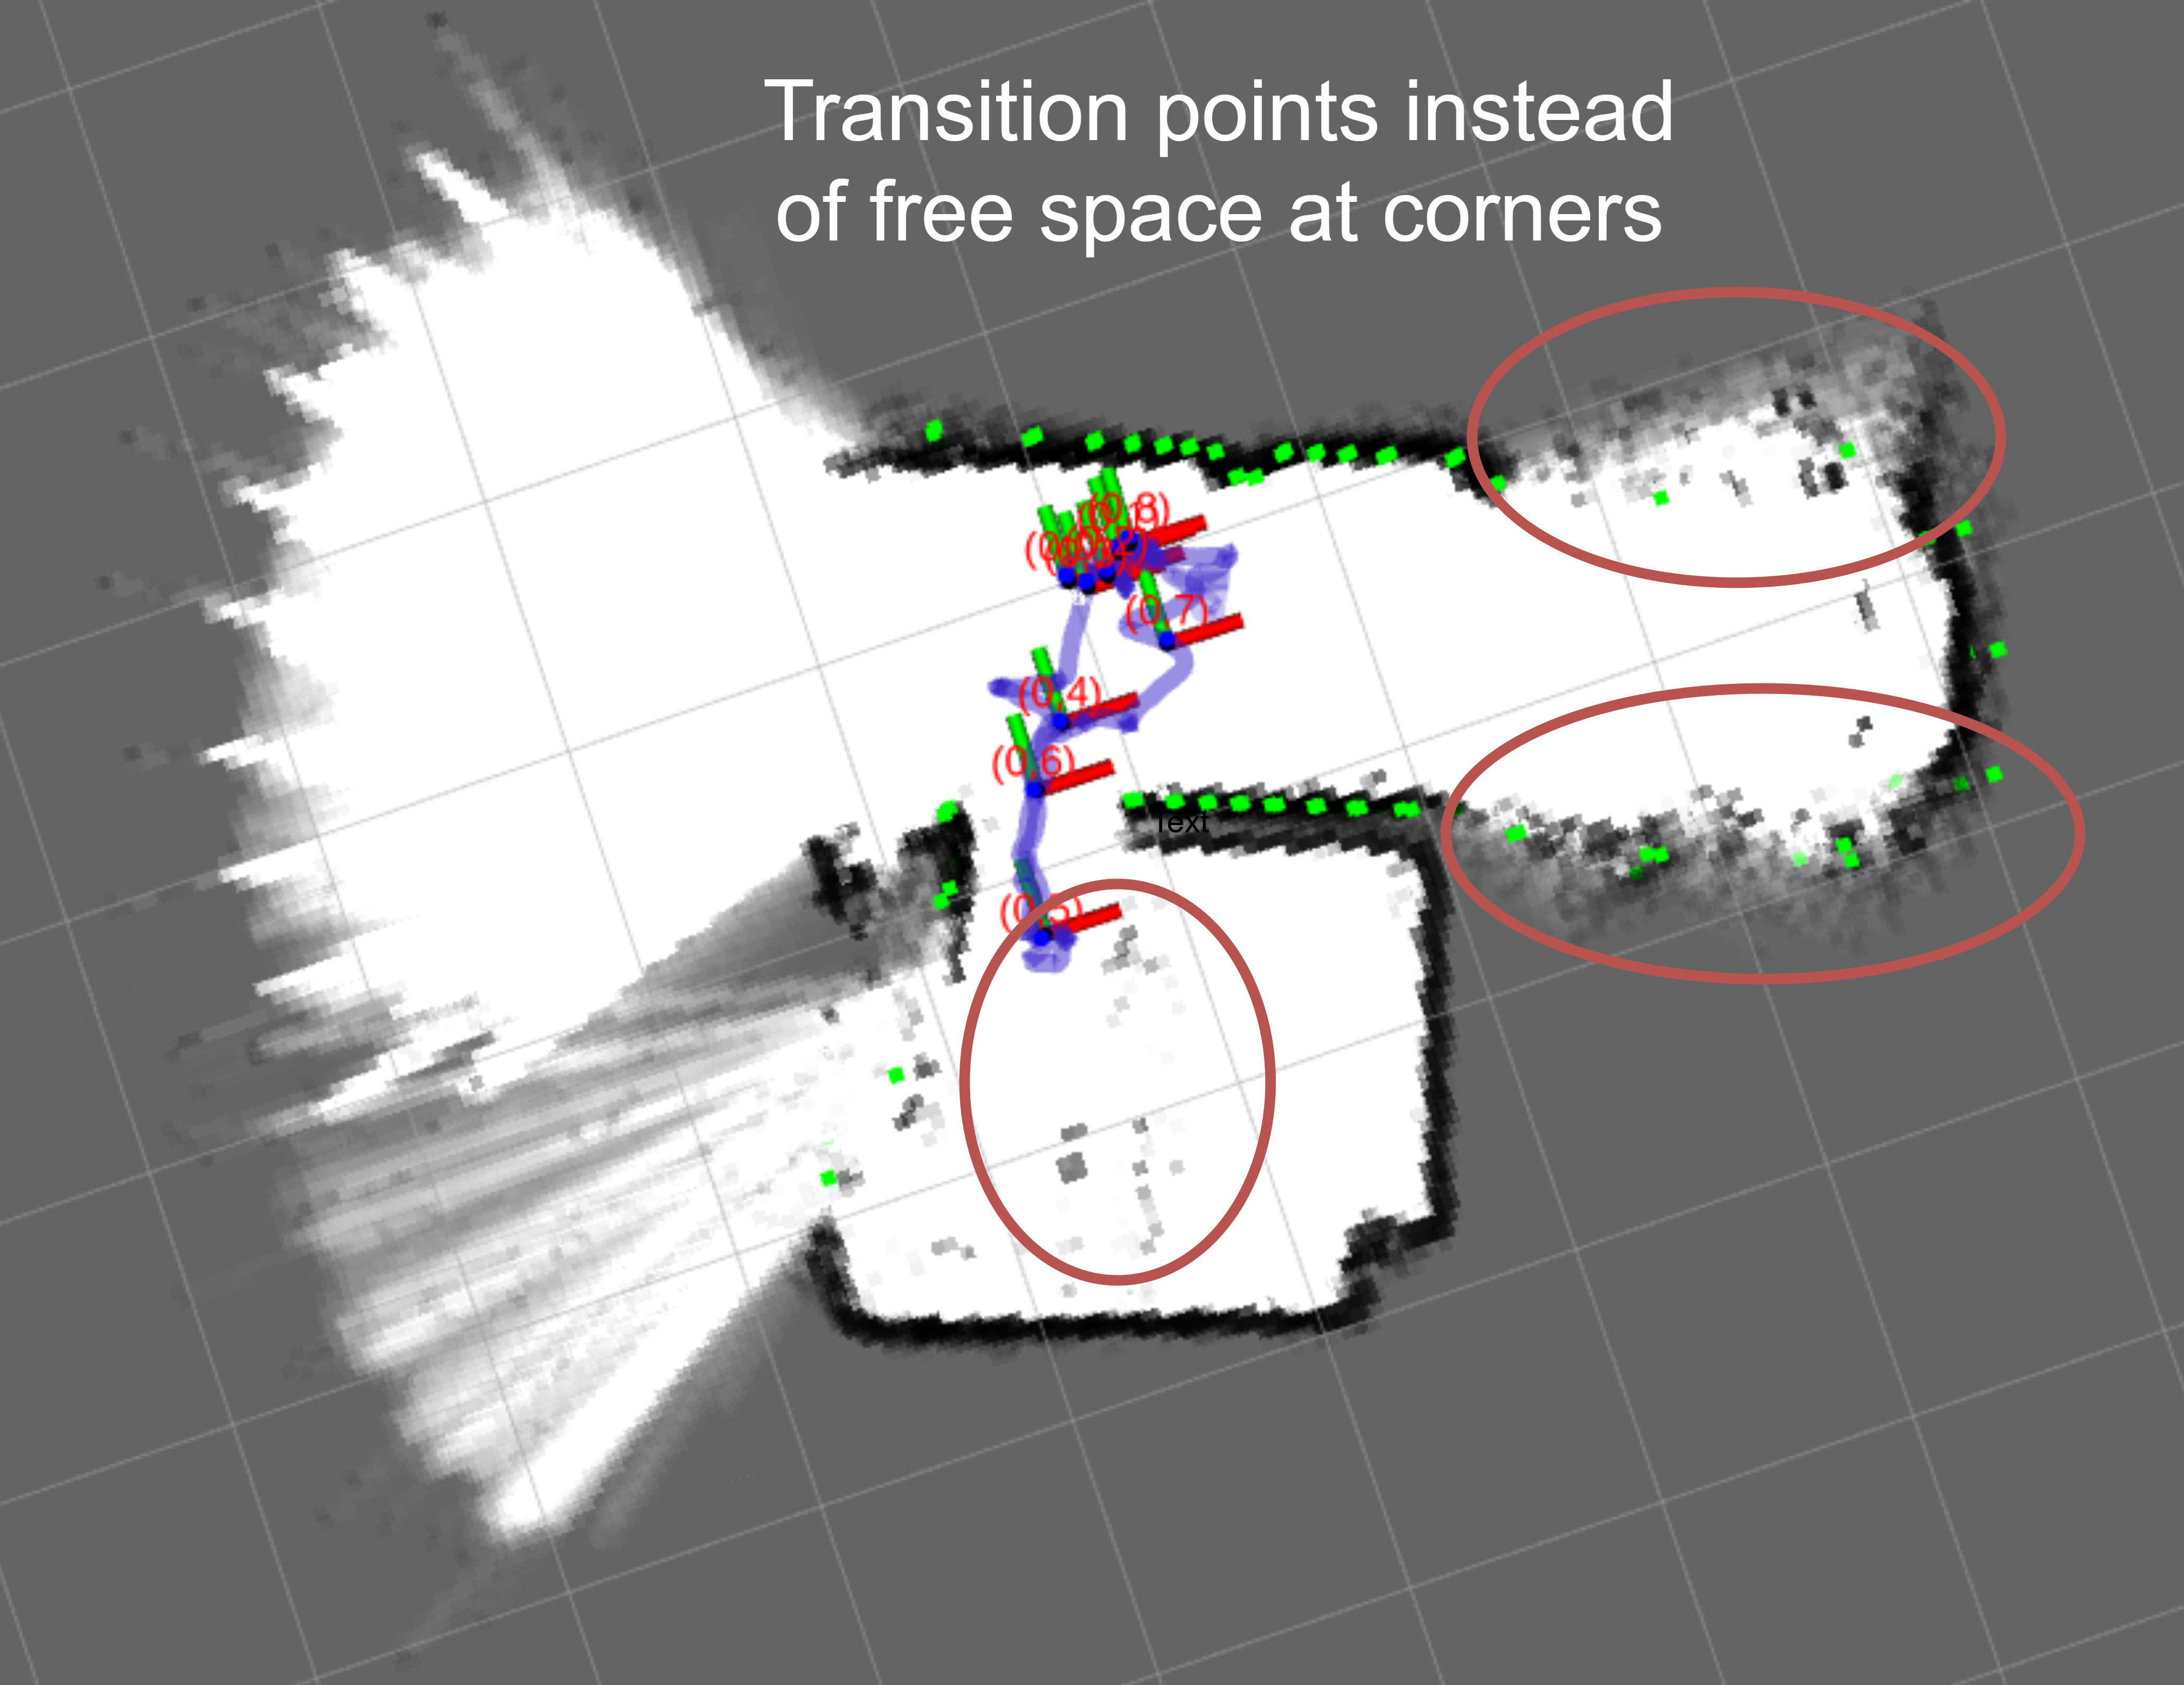
\includegraphics[height=65mm, keepaspectratio]{figures/03_artifacts.png}
    \caption{With wider field of view, the number of transition points increase}
    \label{fig:03_artifacts}
\end{figure}

The tuned SLAM algorithm with sensors at a resolution of 3x3 seems to be stable and produces a
decent quality map. On the way back submaps started to drift in orientation compared to the
already inserted submaps, but global SLAM was able to compensate it and pulled submaps together.
Another artifact is the number of scans that could not be properly inserted into any submap and
therefore produce a tilted shadow of the wall in the top right corner of the map.

\begin{figure}[!h]
    \centering
	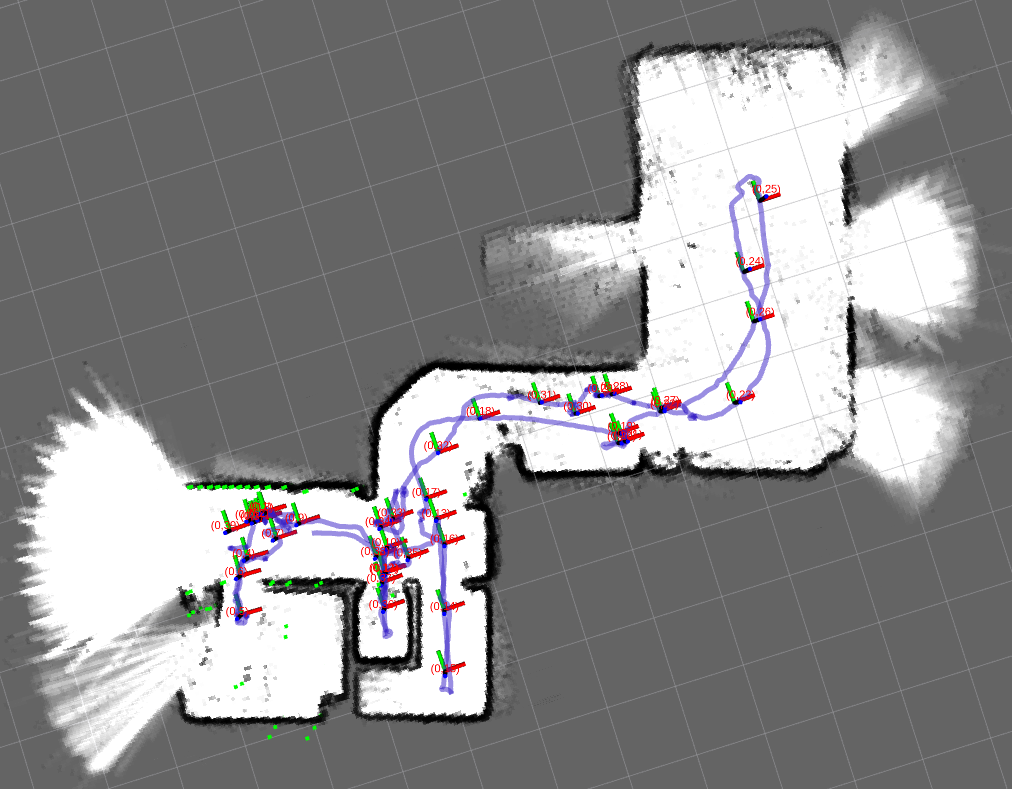
\includegraphics[height=65mm, keepaspectratio]{figures/03_map.png}
    \caption{Map produced by sensors on 3x3-resolution}
    \label{fig:03_map}
\end{figure}

Although the mapping accuracy is reduced with the reduced sensor resolution, the localization
accuracy has increased. The cumulated RMS error for this setup is 11.34cm. The RMS error on the
x- is 4.04cm and on the y-axis it is 7.3cm.

\begin{figure}[!h]
    \centering
	$\vcenter{\hbox{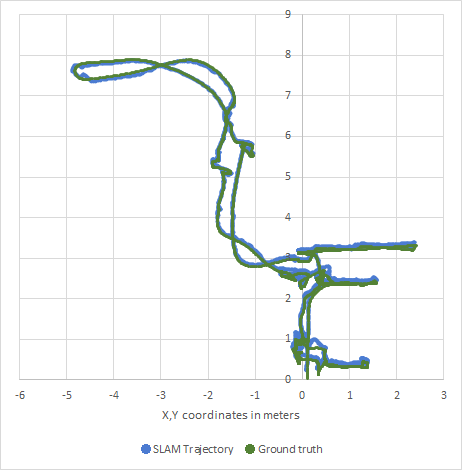
\includegraphics[height=65mm, keepaspectratio]{figures/03_trajectory.png}}}$
    $\vcenter{\hbox{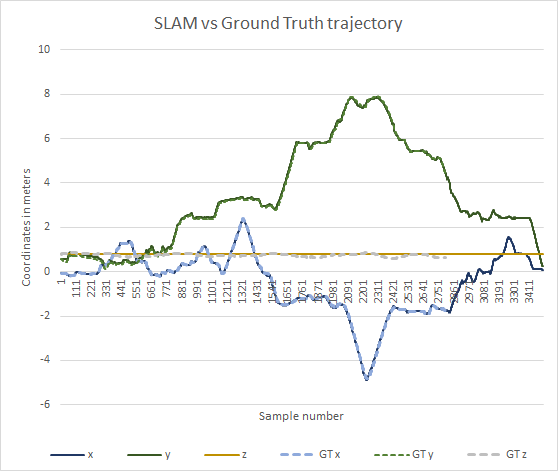
\includegraphics[height=65mm, keepaspectratio]{figures/03_trajectory_coordinates.png}}}$
    \caption{2D SLAM extracted trajectory against ground truth using 3x3-resolution sensors}
    \label{fig:03_trajectory}
\end{figure}

\begin{figure}[!h]
    \centering
	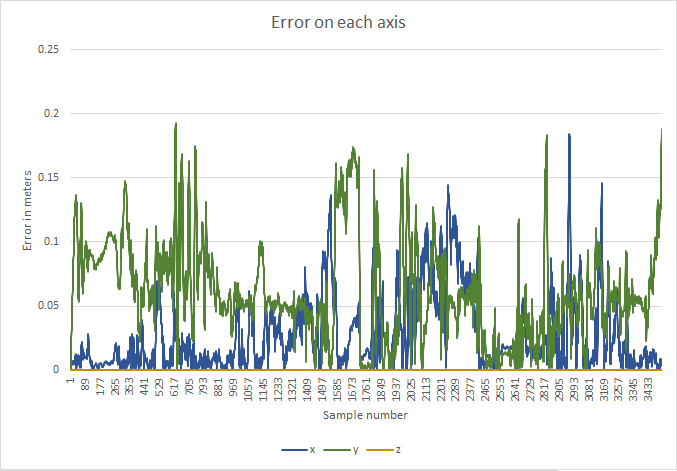
\includegraphics[height=65mm, keepaspectratio]{figures/03_trajectory_error.png}
    \caption{Trajectory error on each axis using 3x3-resolution sensors}
    \label{fig:03_trajectory_error}
\end{figure}

The accuracy of this setup is unexpected because it contains fewer points per scan and more
the presence of transition points is significantly higher. I think the higher accuracy is due
to the better tuning of Cartographer, because and shows the flaw of manual tuning and visual
inspection. It also shows the importance of tuning.






\subsubsection{2D SLAM with 2x2-resolution}
Compared to 3x3-resolution, in 2x2 each scan contains 66\% fewer points. A complete scan of 13
sensors consist of only 52 points, which makes scan matching significantly less efficient.
Tuning of this setup was noticeably harder and the quality of the produced map has highly
decreased.

To compensate for the scarce ranges inside scans, I have also run the simulation with a lowered grid
resolution from 5cm to 15cm. The difference between the two produced maps is seen in figure \ref{fig:04_map}.
The lowered resolution resulted in a more consistent map, but the transient points are also better
visible on this map.

\begin{figure}[!h]
    \centering
	$\vcenter{\hbox{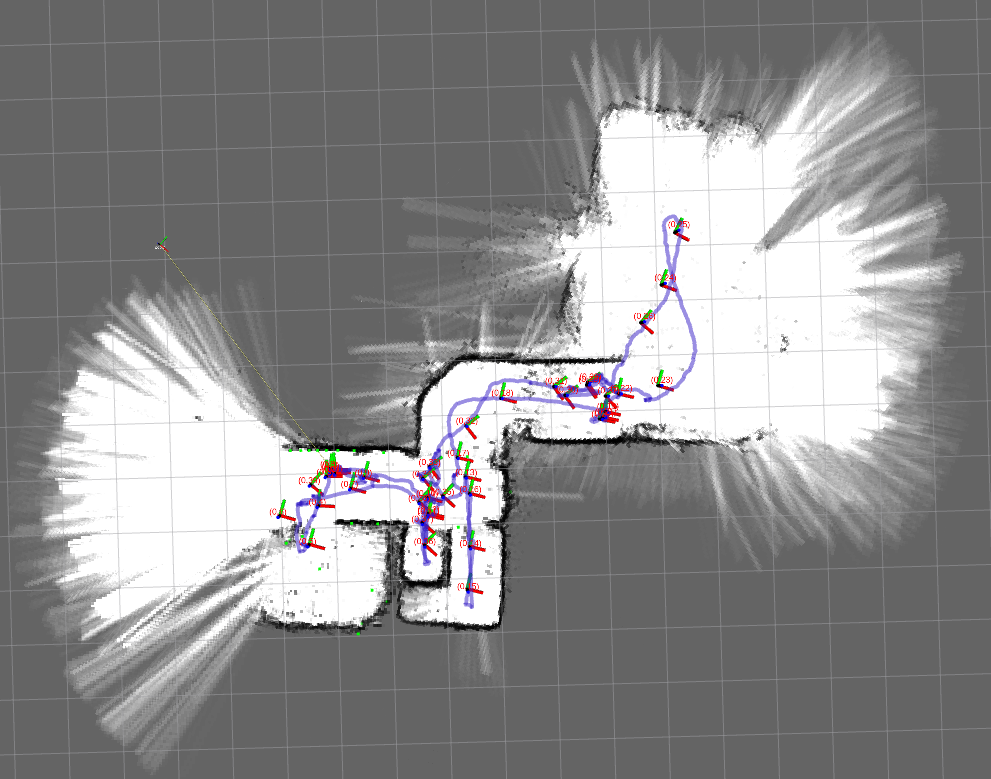
\includegraphics[height=55mm, keepaspectratio]{figures/04_map.png}}}$
    $\vcenter{\hbox{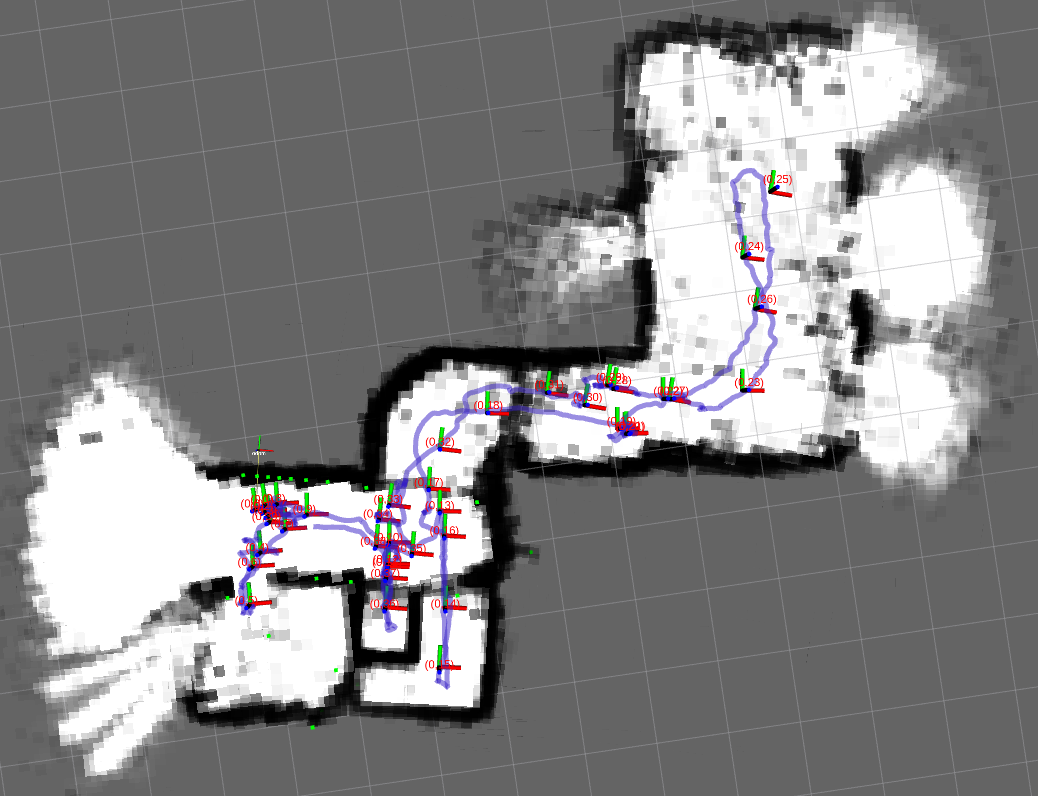
\includegraphics[height=55mm, keepaspectratio]{figures/04_map_lowres.png}}}$
    \caption{Produced map using 5cm grid resolution on the left and 15cm on the right
    using 3x3-resolution sensors}
    \label{fig:04_map}
\end{figure}

By placing the trajectories side by side as in figure \ref{fig:04_trajectory}, the difference is
can be easily seen. While the configuration with a high-resolution grid map is able to follow the ground-truth-trajectory
 in small rooms and the narrow corridor, it loses track in the big and spacious room, when the
ranges are far apart. The lower resolution makes the SLAM algorithm more efficient mostly in the big room but
also has less drift and it is more stable.

\begin{figure}[!h]
    \centering
	$\vcenter{\hbox{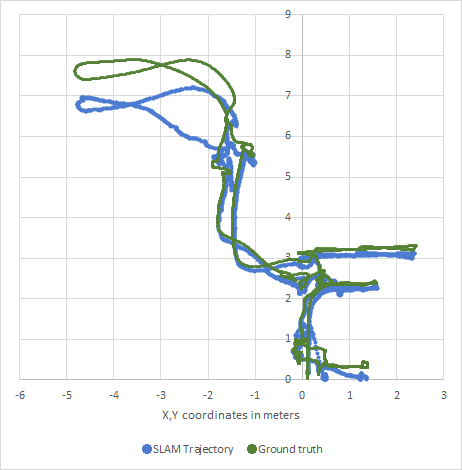
\includegraphics[height=65mm, keepaspectratio]{figures/04_trajectory.png}}}$
    $\vcenter{\hbox{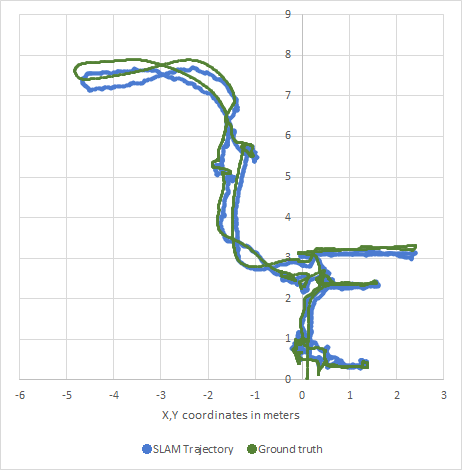
\includegraphics[height=65mm, keepaspectratio]{figures/04_trajectory_lowres.png}}}$
    \caption{Comparison of estimated trajectories using 5cm grid resolution on the left and 15cm
    on the right}
    \label{fig:04_trajectory}
\end{figure}

The high-resolution trajectory is at some points as far as 1.4m from the ground-truth pose, but the
cumulated RMS error is only 43.4cm. This shows that a seemingly small difference in RMS error can mean
an error of more than a meter at a part of the trajectory. The low-resolution trajectory in comparison
has a cumulated RMS error of 22.13cm. 7.95cm error on the x- and 14.17cm on the y-axis.

\begin{figure}[!h]
    \centering
	$\vcenter{\hbox{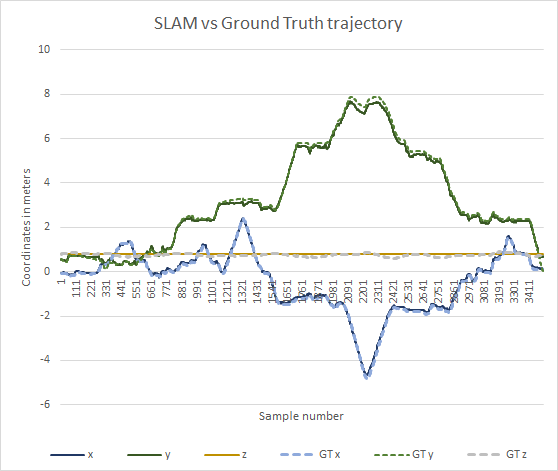
\includegraphics[height=55mm, keepaspectratio]{figures/04_trajectory_lowres_coordinates.png}}}$
    $\vcenter{\hbox{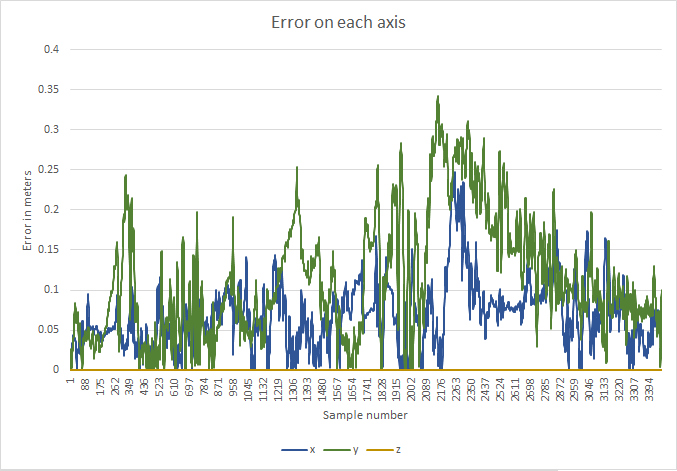
\includegraphics[height=55mm, keepaspectratio]{figures/04_trajectory_lowres_error.png}}}$
    \caption{2D SLAM extracted trajectory against ground truth using 2x2-resolution sensors and
    15cm grid resolution}
    \label{fig:04_trajectory_lowres}
\end{figure}





\subsubsection{2D SLAM with 1x1-resolution}
By further lowering the resolution, each sensor has a single range measurement as output resulting in 13
range measurements per a complete scan. Such a low-resolution hides most of the details and almost always
has multiple walls in its field of view. For example, on 4m distance with a 27$^{\circ}$ angle, the field of
view opens to 1.8m. All ranges inside this wide field of view get averaged, which results in one distance
measurement. On the corridor the drone flies in, ranges of a single sensor's scan can hit the two parallel
walls and also the wall at the end of the corridor. This scan will produce a floating-point in the middle
of the corridor.

Due to the high rate of the above-mentioned artifacts, I was not able to tune the SLAM algorithm. With all
settings tried, the system proved to be unstable and unreliable.





\subsubsection{Summary}
After running and tuning the SLAM algorithm on all resolutions, I can conclude that higher resolutions
positively affect the stability and reliability of Cartographer. Lower resolution means a broader field of
view that hides details like corners and edges, resulting in poorer quality maps.

Table \ref{tab:error_on_different_resolutions} shows the the RMS error for each resolutions I have tried.
Surprisingly the setup with 3x3 sensors has a smaller RMS error, than the unfiltered setup or 4x4 setup.
The reason for this might be because I have conducted these experiments in the same order as in this document
and I have gained more experience in the tuning of Cartographer by the time I have got to the experiment with 3x3-resolution
sensors.

\begin{table}[ht]
	% \footnotesize
	\centering
	\begin{tabular}{||c c c c c c||}
		\hline
                            & Unfiltered    & 4x4     & 3x3     & 2x2     & 1x1 \\
		\hline\hline
        RMS error on x axis & 6.3cm         & 8.12cm  & 4.04cm  & 7.95cm  & -\\
        \hline
        RMS error on y axis & 6.5cm         & 10.48cm & 11.34cm & 14.17cm & -\\
		\hline
        Cumulated RMS error & 12.8cm        & 18.6cm  & 15.74cm & 22.13cm & -\\
		\hline
	\end{tabular}
	\caption{RMS error on different resolutions}
	\label{tab:error_on_different_resolutions}
\end{table}






\subsection{Effects of sampling rate}
In the investigation of the effects of the sampling rate, only two resolutions with the lowest RMS error
are used. These resolutions are 4x4 and 3x3. In this test, the same LIDAR layout is kept as before,
13 sensors evenly placed on the horizontal axis. Only one parameter is changed, that is the sampling
rate of each sensor.

For 4x4-resolution I chose the sampling time at 400ms, based on the measurements in section
\ref{sect:vl53l1x_detailed_measurements}. I chose the setup with a timing budget of 33ms over 18.5ms
because it has a lower sampling rate and if it works using this setting, it should be working with
a higher sampling rate too.

As for 3x3-resolution, I chose the setup with the same sampling rate of 33ms. This setup has a sampling
time of 220ms.






\subsubsection{4x4-resolution}
The dropped sampling rate from 30Hz to 2.5Hz is significant and makes tuning much harder. In previous
simulations, the occupied\_space\_weight parameter was not at all or only slightly changed, but in this,
case this parameter proved to be the key parameter. This parameter sets how heavily Cartographer should
rely on already inserted points. The higher this value, the less flexible already inserted points are and
are less likely to be overwritten by new scans.

As seen in the previous simulation that uses 2x2-resolution sensors, I have also tried in this case
to lower the grid resolution to 15cm. The two completed maps are seen in figure \ref{fig:05_maps}.
The quality of the map is decent in both cases, no major flaw is visible. In both cases, global SLAM
had to compensate rotation drifts, that occurred when the drone turned around in the big room. This
was in general a crucial point in the tuning procedure, most often submaps fell apart at this point.

\begin{figure}[!h]
    \centering
	$\vcenter{\hbox{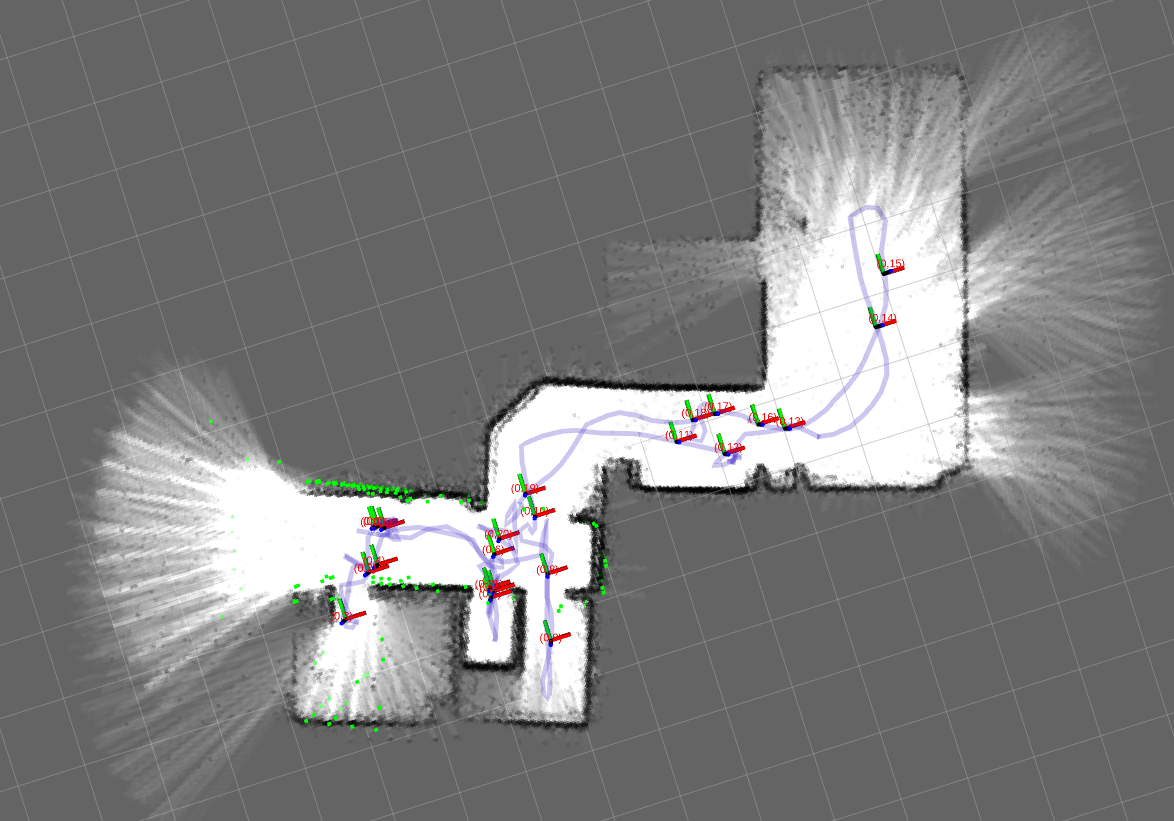
\includegraphics[height=50mm, keepaspectratio]{figures/05_map_highres.png}}}$
    $\vcenter{\hbox{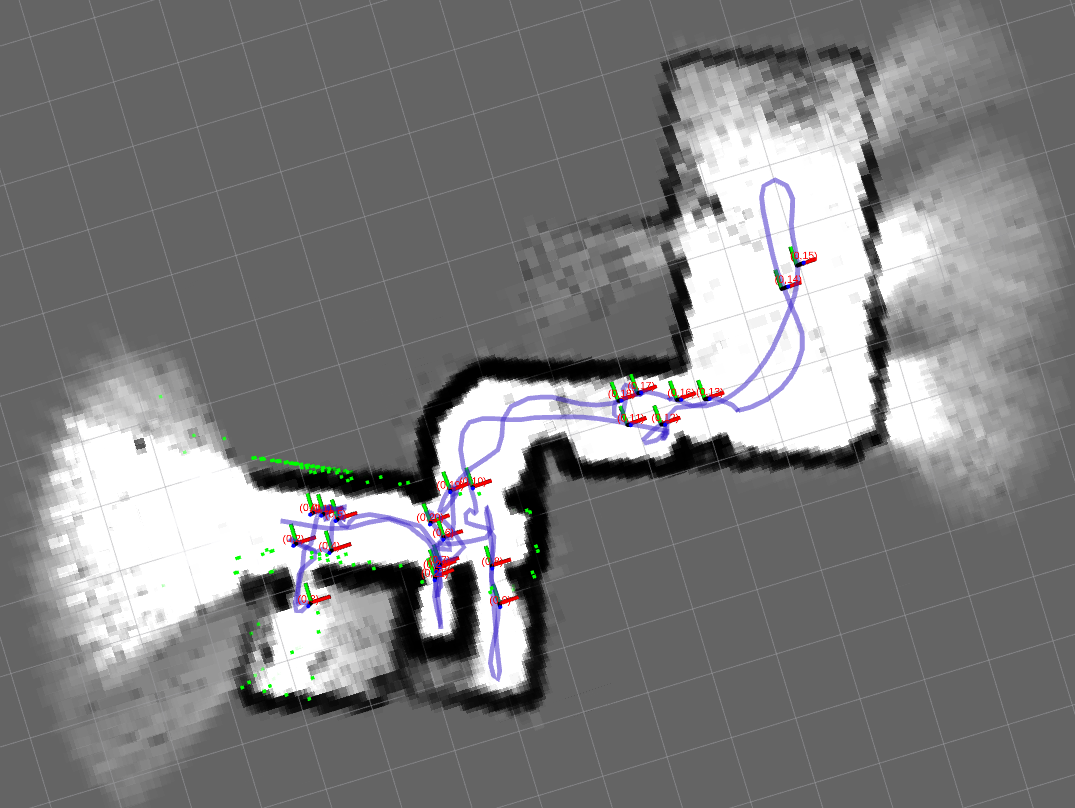
\includegraphics[height=50mm, keepaspectratio]{figures/05_map_lowres.png}}}$
    \caption{Maps built using 4x4-resolution sensors. 5cm grid resolution on the left and
    15cm resolution on the right}
    \label{fig:05_maps}
\end{figure}


The two trajectories \ref{fig:05_trajectory} look similar, both follow the ground-truth trajectory
closely. Low grid resolution produces a smoother path, while on high-resolution there are some
edges and sharper turns. In general, the configuration with a 5cm grid resolution felt very unstable
and that it can fall apart at any point. If submaps are built properly but misplaced relative to
each other, it can still be compensated by global SLAM, but in this case, submaps fell apart, which
cannot be compensated anymore.

\begin{figure}[!h]
    \centering
	$\vcenter{\hbox{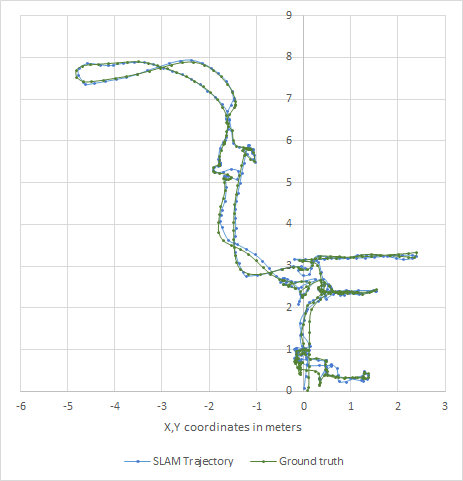
\includegraphics[height=65mm, keepaspectratio]{figures/05_trajectory.png}}}$
    $\vcenter{\hbox{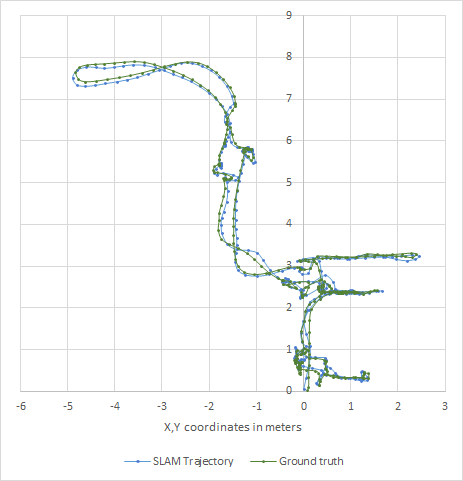
\includegraphics[height=65mm, keepaspectratio]{figures/05_trajectory_lowres.png}}}$
    \caption{Extracted trajectories using 4x4-resolution sensors. 5cm grid resolution on the left
    and 15cm grid resolution on the right}
    \label{fig:05_trajectory}
\end{figure}

The cumulated RMS error on a 5cm grid resolution is 16.49cm, on 15cm resolution it is higher: 18.95cm.
Higher grid-resolution results in greater accuracy in position estimates, but its stability is lower
in comparison to lower resolution.


\subsubsection{3x3-resolution}
The benefit of using a 3x3-resolution setting for the LIDAR is the higher sampling rate. Using the
same timing budget of 33ms as for 4x4-resolution, the sampling time is 220ms in comparison to the
previous 400ms. This results in an 80\% increase in update rate to 4.5Hz, which also means almost twice
more often pose updates.

Due to high instability, I was unable to tune SLAM with a 5cm grid resolution. Lowering the grid
resolution once again to 15cm, resolved the issue and the system felt reliable afterward. The
produced map using a higher grid size is in figure \ref{fig:06_trajectory}. The map quality is
adequate, global SLAM almost hasn't done any corrections.


\begin{figure}[!h]
    \centering
	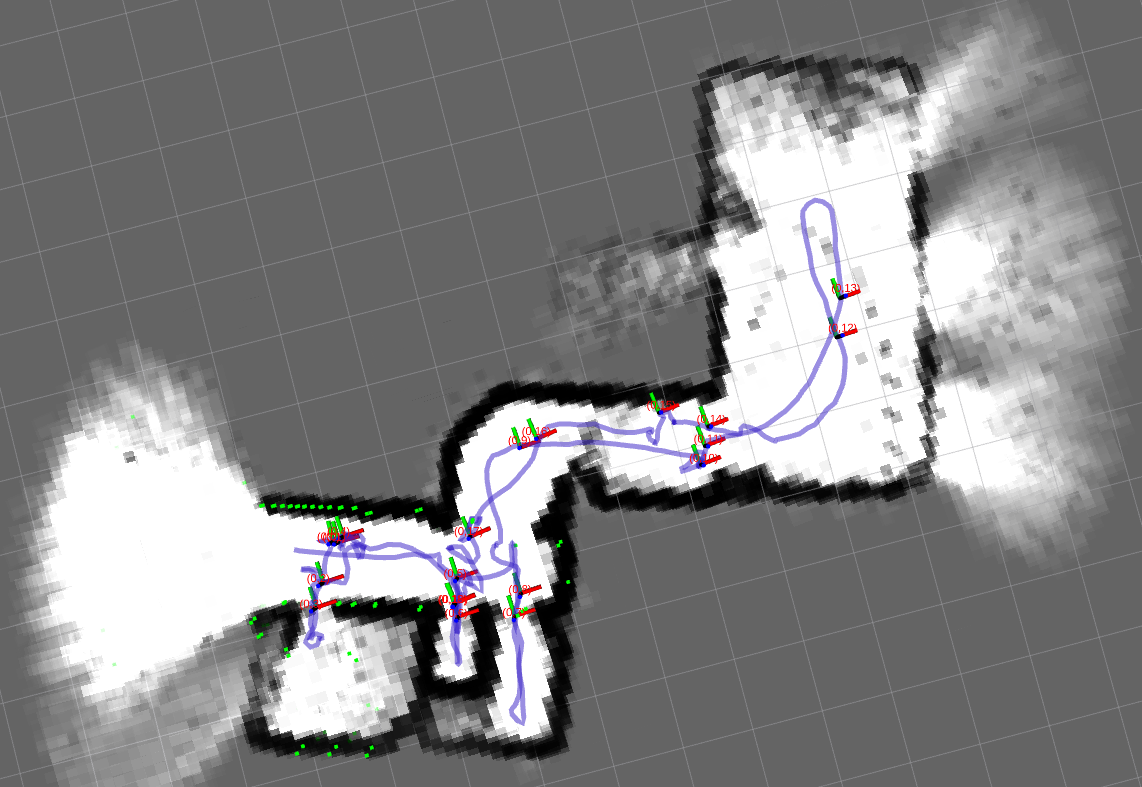
\includegraphics[height=50mm, keepaspectratio]{figures/06_map.png}
    \caption{Map built using 3x3-resolution sensors and 220ms sampling time}
    \label{fig:06_map}
\end{figure}

The extracted trajectory is seen in figure \ref{fig:06_trajectory}. The cumulated RMS error is
14.67cm, 6.4cm on the x-axis, and 8.2 on the y-axis. Based on the stability and also accuracy 3x3-resolution
seems like a better resolution for Cartographer SLAM.

\begin{figure}[!h]
    \centering
	$\vcenter{\hbox{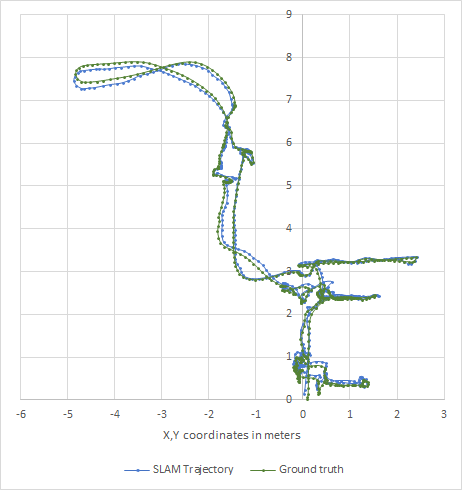
\includegraphics[height=65mm, keepaspectratio]{figures/06_trajectory.png}}}$
    $\vcenter{\hbox{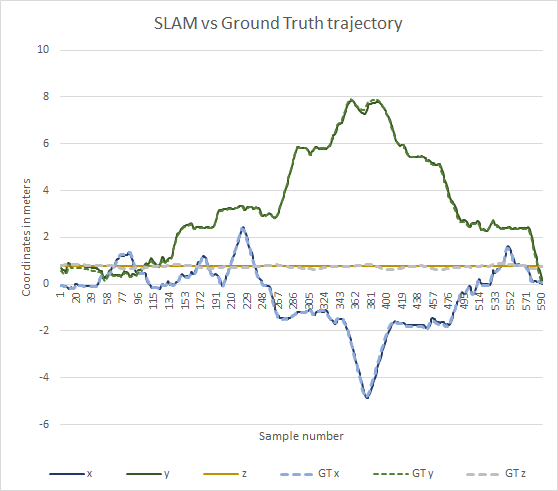
\includegraphics[height=65mm, keepaspectratio]{figures/06_trajectory_coordinates.png}}}$
    \caption{Extracted trajectory using 3x3-resolution sensors and 220ms sampling rate}
    \label{fig:06_trajectory}
\end{figure}

\subsection{Effects of maximum distance} \label{sect:effects_of_max_dist}
The measurements with the VL53L1X sensor showed that each setup works accurately until 2.5m and each
has about 25cm drift at a distance of 3m. I chose 2.75m as maximum distance for both 3x3 and 4x4-resolution
sensor simulations, because this is the distance reported by the sensor on 3m.

The lowered maximum distance had a positive effect, that the number of transition points has been
reduced. This is because the shorter distance means that the field of view is shortened and cannot
open as wide as it could before. The downside of the limited range is that the algorithm loses track
in the big room because it's longer than 5m and the two farther sides do not fit in a single scan.
This caused more flaws in 4x4-resolution, while the other map looks similar to the one before
the introduction of the distance limit. A small tilt can be observed that there is a slight tilt
between the room on the right and the rest of the map. The produced maps using both 3x3 and 4x4
resolution setups are in figure \ref{fig:07_map}.


\begin{figure}[!h]
    \centering
	$\vcenter{\hbox{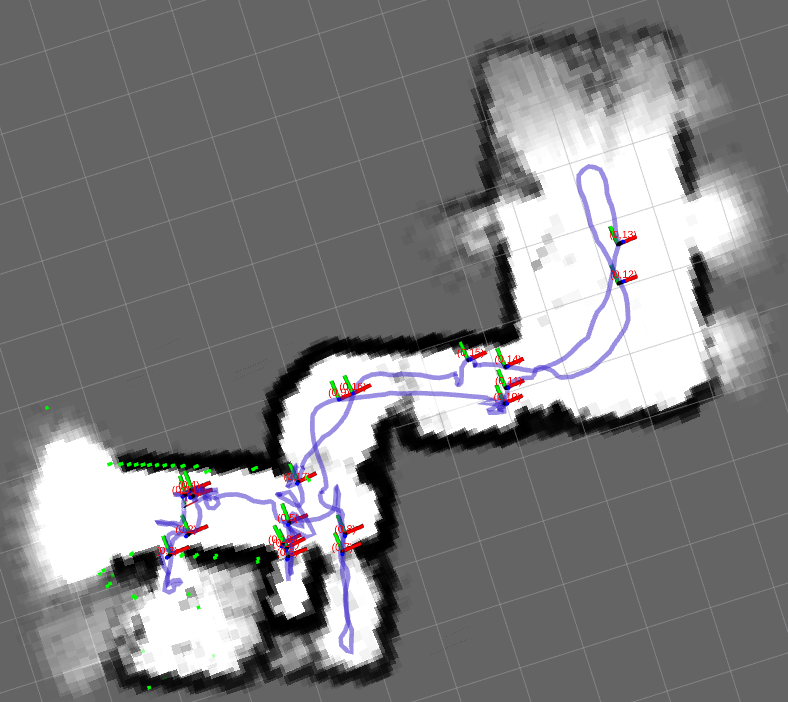
\includegraphics[height=50mm, keepaspectratio]{figures/07_map_3x3_2_75d.png}}}$
    $\vcenter{\hbox{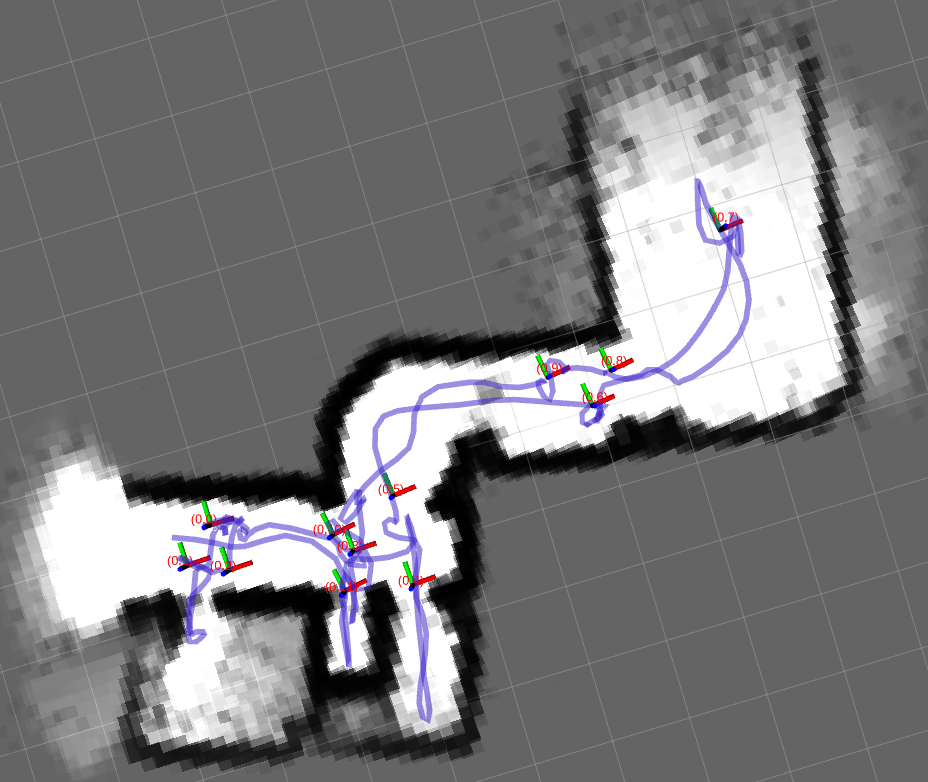
\includegraphics[height=50mm, keepaspectratio]{figures/07_map_4x4_2_75d.png}}}$
    \caption{Maps produced by SLAM algorithm with 2.75m maximum distance and realistic sampling rate
    enabled, 3x3-resolution on the left, 4x4-resolution on the right}
    \label{fig:07_map}
\end{figure}

The trajectory using sensors with 3x3-resolution has a significant offset on the y-axis, that appeared
after the drone exited the very first room. This offset is picked up because with the maximized distance
the corridor appears to be open on both ends and without any reference points. Similar scans are pulled
together, resulting in a shortened corridor.


\begin{figure}[!h]
    \centering
	$\vcenter{\hbox{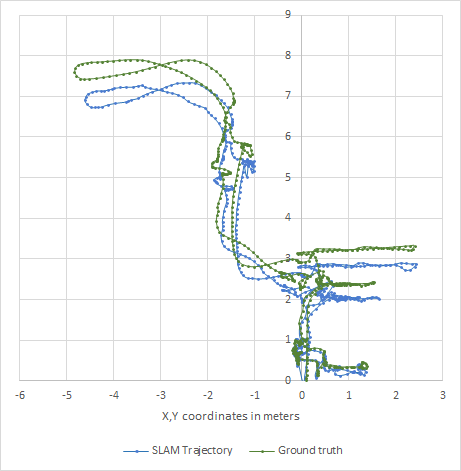
\includegraphics[height=65mm, keepaspectratio]{figures/07_trajectory_3x3.png}}}$
    $\vcenter{\hbox{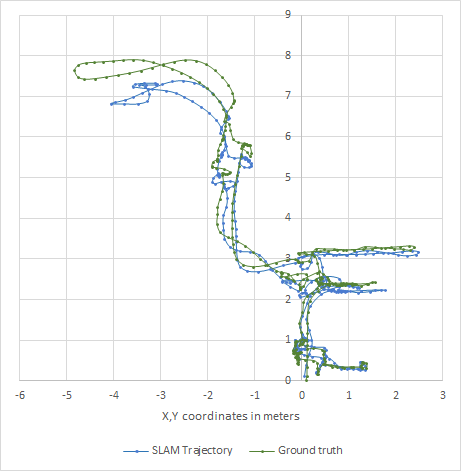
\includegraphics[height=65mm, keepaspectratio]{figures/07_trajectory_4x4.png}}}$
    \caption{Extracted trajectories with 2.75m maximum distance and realistic sampling rate,
    3x3-resolution on the left and 4x4-resolution on the right}
    \label{fig:07_trajectories}
\end{figure}

The trajectory using the setup with 4x4-resolution sensors has a smaller offset. It seems like with
more points per scan the SLAM algorithm was able to pick up small details and better track the
movement of the drone on this mostly even corridor. On the other hand, it failed in the big room,
where the same situation appears. The stairs at the end of the room also make tracking harder.
Ranges from the stairs and the wall are hard to differentiate.

The cumulated RMS error for 3x3-resolution is 45cm and 49.6cm for 4x4. In the end the mostly
constant offset with otherwise correct shape results in a smaller error, than the pose estimation
that follows ground-truth closely but fails in shape at a relatively small area.




\subsection{Reduced set of evenly distributed LIDAR sensors}
The goal is to find the minimum number of LIDAR sensors, with which the SLAM algorithm still
works reliably and can produce a coherent map. To see the effect of reduction in the number of
sensors, I have decided to halve the set and test the performance using only 6 sensors. The
sensors are evenly placed to cover the 360$^{\circ}$ horizontal plane.

\begin{figure}[!h]
    \centering
	$\vcenter{\hbox{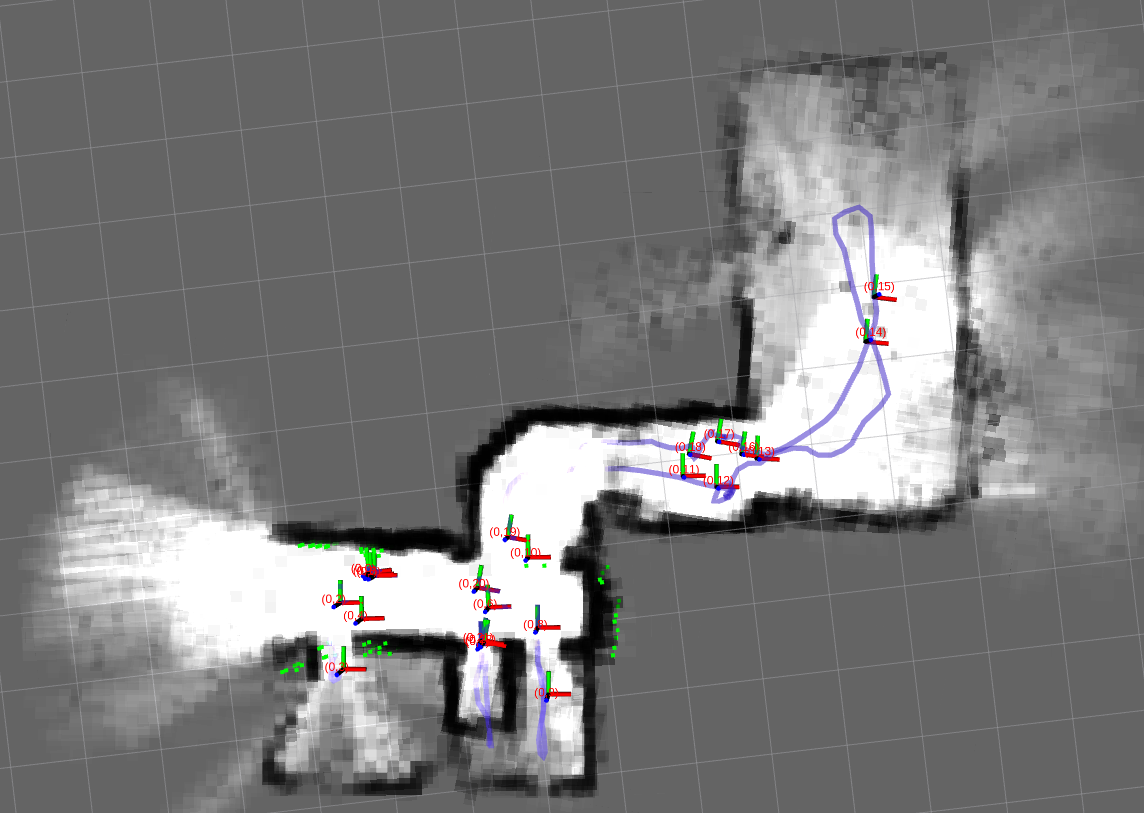
\includegraphics[height=50mm, keepaspectratio]{figures/08_map_unlimited.png}}}$
    $\vcenter{\hbox{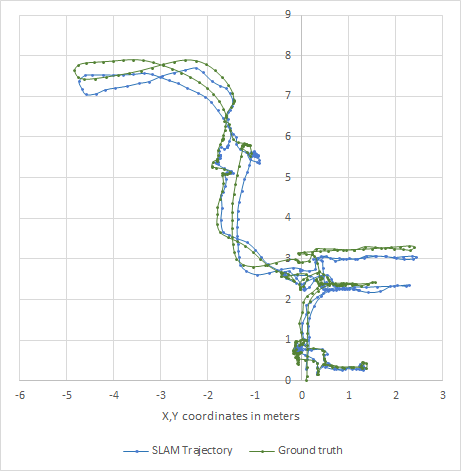
\includegraphics[height=50mm, keepaspectratio]{figures/08_trajectory_unlimited.png}}}$
    \caption{Map and trajectory using 6 pieces of 4x4-resolution sensor with a 400ms sampling time
    and 4m distance limit}
    \label{fig:08_map_unlimited}
\end{figure}

At first, I used 4x4-resolution sensors with a 400ms update rate and without limiting the maximum
distance. This means the maximum distance of each sensor is 4m.
The produced map is almost as good as it was with 13 sensors, but the tuning was difficult
and it was sensitive to any small changes in weights. The cumulated RMS error of this setup is
37.32cm.


\begin{figure}[!h]
    \centering
	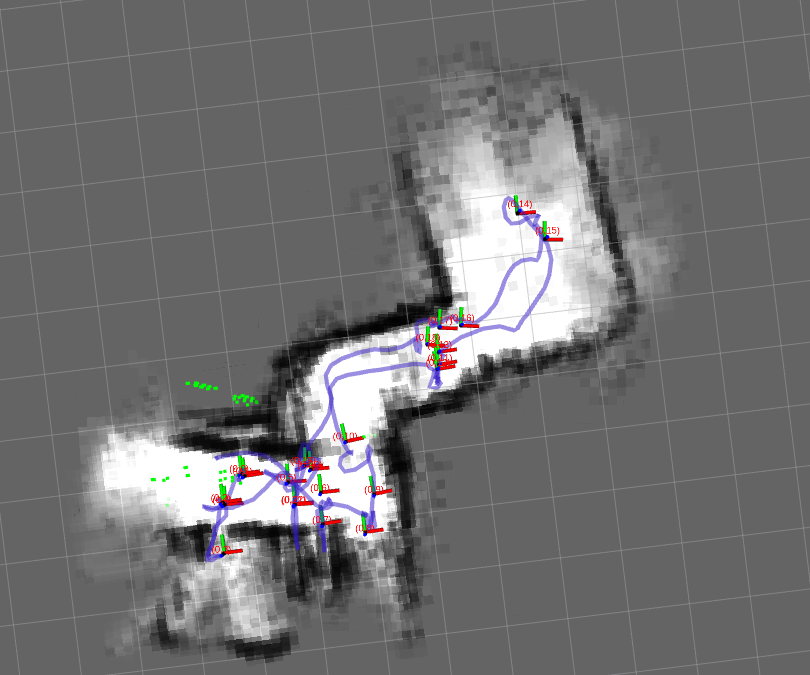
\includegraphics[height=50mm, keepaspectratio]{figures/08_failed_map.png}
    \caption{Failed mapping attempt with 4x4-resolution, 400ms sampling time and 2.75m
    maximum distance}
    \label{fig:08_failed_map}
\end{figure}


After tuning the setup without distance filter, I have used the same number of sensors and layout
with distance filter enabled. The maximum distance is set to 2.75m as in previous simulations.
The tuning of the algorithm proved to be significantly harder this time. In the end, I couldn't
find any combination of parameters that would enable the mapping to work reliably.
Due to the low number of sensors, there are not enough remarkable details in scans that would
enable proper scan matching.
The best produced map using 4x4-resolution sensors is in figure \ref{fig:08_failed_map}.
Similar maps were created using 3x3-resolution.

\begin{figure}[!h]
    \centering
	$\vcenter{\hbox{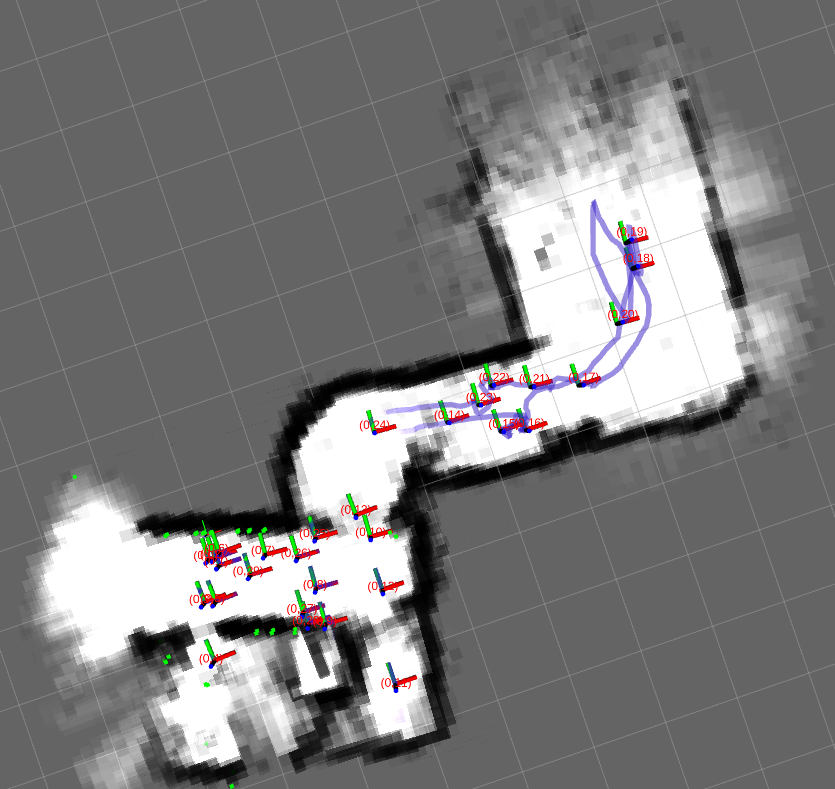
\includegraphics[height=50mm, keepaspectratio]{figures/08_map_8sensor_3x3.png}}}$
    $\vcenter{\hbox{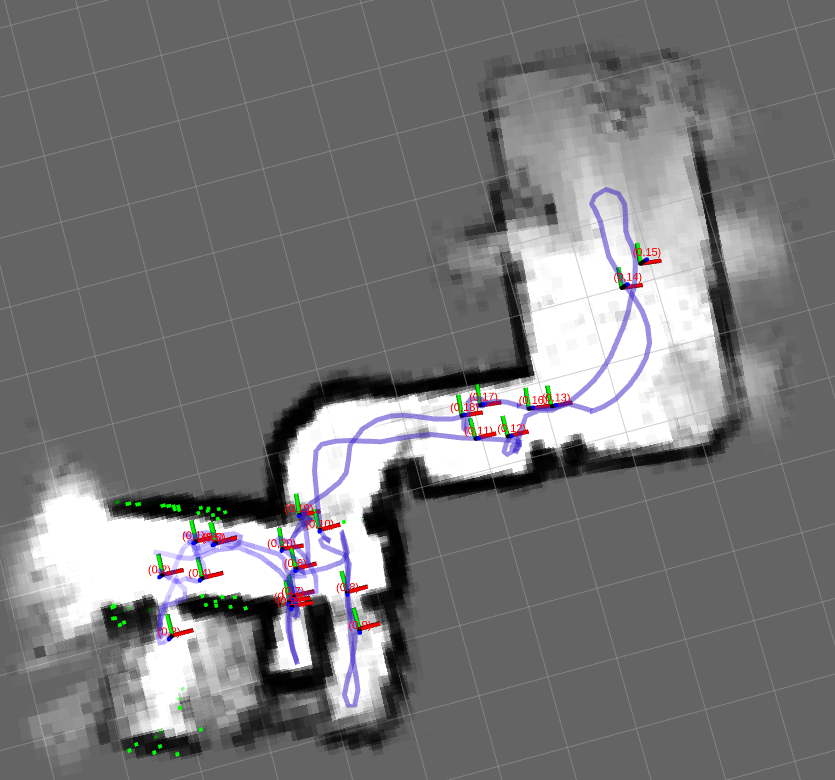
\includegraphics[height=50mm, keepaspectratio]{figures/08_map_8sensor_4x4.png}}}$
    \caption{SLAM maps using 8 sensors in even layout, realistic sampling time, 2.75m distance limit,
    3x3-resolution on the left and 4x4 on the right}
    \label{fig:08_map_8_sensors}
\end{figure}

After the failed attempt using 6 sensors, I have raised the number to 8 and filtered the original
bag using 3x3 and 4x4-resolution. The increased number had a positive effect and I was able to
tune the algorithm properly. In contrary to the measurements in \ref{sect:effects_of_max_dist},
this time setup using 4x4-resolution successfully tracked the drone even in the big room,
while 3x3-resolution failed.


RMS cumulated error using 8 sensors with 4x4-resolution is 34.1cm and almost triple 89.5cm
using 3x3-resolution. The extracted trajectories can be inspected in figure \ref{fig:08_8p_trajectories}.
In different quantities, but both trajectories have an offset that cumulated after exiting the first
room, due to the shortening of corridors. This offset persists throughout the trajectories afterward,
but the submaps are properly aligned relative to each other.

\begin{figure}[!h]
    \centering
	$\vcenter{\hbox{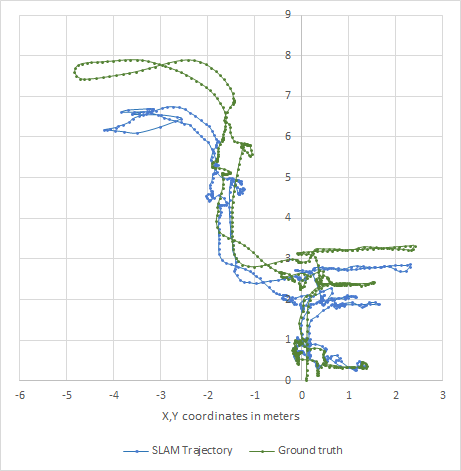
\includegraphics[height=65mm, keepaspectratio]{figures/08_trajectory_8p_3x3.png}}}$
    $\vcenter{\hbox{\includegraphics[height=65mm, keepaspectratio]{figures/08_trajectory_8p_4x4.png}}}$
    \caption{SLAM trajectories using 8 sensors in even layout, realistic sampling time, 2.75m distance limit,
    3x3-resolution on the left and 4x4 on the right}
    \label{fig:08_8p_trajectories}
\end{figure}

I have tried to lower the number of sensors to 7, but I have got the same results as with 6 sensors.
Therefore the setup using 8 sensors is assumed to be the lowest number of VL53L1X sensors, that is still
able to produce consistent maps with Cartographer SLAM in 2D mode.


\newpage

\section{3D SLAM evaluation}
To evaluate the 3D SLAM performance, I decided to work towards the minimum number of LIDAR sensors in
incremental steps, just like in the case of 2D. 3D SLAM is an extension of 2D SLAM and most concepts learned
in 2D apply to it. Nevertheless, 3D SLAM is significantly more complex and tuning procedure is harder due
to the larger number of configuration parameters. Rviz can only visualize the 2D projection of the 3D
map, this will be used as a base for tuning.

For the first simulation, I have converted the PointCloud messages but left data unfiltered to see the
maximum accuracy of the 3D SLAM algorithm using unfiltered data.

To see the effects of resolution, sampling rate and maximum distance I have used 43 sensors with
4x4-resolution and introducing the according parameters incrementally. In the layout 13 sensors pointing
at 0$^{\circ}$, 9-9 at $\pm$30$^{\circ}$, 5-5 at $\pm$60$^{\circ}$ and 1-1 at $\pm$90$^{\circ}$ all
relative to the horizontal plane and evenly placed around the vertical axis as in figure \ref{fig:09_layout}.

\begin{figure}[!h]
    \centering
	\includegraphics[height=50mm, keepaspectratio]{figures/09_layout.png}
    \caption{Visualization of ranges inside field of views of 43 sensors without averaging applied}
    \label{fig:09_layout}
\end{figure}

The 3D SLAM evaluation happens in incremental steps. All steps will be tested using a 4x4 sensor resolution
setting because this resolution is expected to have the best performance. After completing all the steps,
3x3-resolution is also evaluated with all parameters introduced at once. Based on the results of the previous
simulations, I try to lower the number of sensors until the produced map is still consistent.




\subsection{Unfiltered data}
As the first step, the same settings need to be set up as used in 2D SLAM. These settings are the
minimum and maximum range, number of range data to accumulate, IMU gravity time constant, but there
is no option to exclude ranges based on elevation.

Cartographer in 3D SLAM mode uses two probability grid resolutions to reduce computation complexity, a
low and a high-resolution. Cartographer, in general, is optimized for LIDAR sensors with a range up to and
above 100m, therefore the low-resolution grid has a large grid size of 45cm. To make it work more
accurately with the selected VL53L1X sensor, I have lowered the low-resolution grid size to 15cm instead.
Finding the right rotation is a computationally expensive operation for the scan matching algorithm, and
for this reason, the rotation\_weight parameter was set to 400. The drone has quick rotations, so the
algorithm needs to compensate for these rotations. To allow rotations I have lowered the rotation\_weight
parameter and found 15 to be an optimal value.


\begin{figure}[!h]
    \centering
	$\vcenter{\hbox{\includegraphics[height=50mm, keepaspectratio]{figures/09_map.png}}}$
    $\vcenter{\hbox{\includegraphics[height=50mm, keepaspectratio]{figures/09_pointcloud.png}}}$
    \caption{3D slam map and inserted points using unfiltered data}
    \label{fig:09_3d_map}
\end{figure}


The estimated trajectory against ground-truth is visible in figure \ref{fig:09_3d_trajectory}. The error of
the estimation is relatively small and it typically stays under 15cm but never goes above 30cm.
The cumulated RMS error for the unfiltered setup is 10.4cm, with 3.6cm error on the x-, 4.4cm on the y- and
2.4cm on the z-axis.


\begin{figure}[!h]
    \centering
	$\vcenter{\hbox{\includegraphics[height=60mm, keepaspectratio]{figures/09_trajectory.png}}}$
    $\vcenter{\hbox{\includegraphics[height=60mm, keepaspectratio]{figures/09_trajectory_coordinates.png}}}$
    \caption{3D slam trajectory using unfiltered data}
    \label{fig:09_3d_trajectory}
\end{figure}

The visualization of the point cloud on these images happened, by setting the decay time parameter to
a high number in Rviz. This way all matched points published by Cartographer will be displayed in
this visualization. These point clouds however do not change with optimization of global SLAM but
stay fixed as the submap was originally inserted. Two more images can be seen, of the visualization,
in figure \ref{fig:09_3d_pointclouds}.

\begin{figure}[!h]
    \centering
	\includegraphics[width=100mm, keepaspectratio]{figures/09_pointcloud2.png}
    \includegraphics[height=60mm, keepaspectratio]{figures/09_pointcloud3.png}
    \caption{3D slam visualization of inserted points in Rviz}
    \label{fig:09_3d_pointclouds}
\end{figure}

Some tilt can be observed relative to the horizontal plane. To see if this tilt is
persistent or has been corrected, the final optimized point cloud can be extracted using
Cartographer's asset writer functionality. After the extraction, the cloud is visualized using Point Cloud
Viewer developed by Google and seen on \ref{fig:09_3d_pointcloud_pcl}. The tilt seems to be optimized
by global SLAM.

\begin{figure}[!h]
    \centering
	\includegraphics[width=100mm, keepaspectratio]{figures/09_pointcloud4.png}
    \caption{3D slam visualization of extracted point cloud in Point Cloud Viewer}
    \label{fig:09_3d_pointcloud_pcl}
\end{figure}




\subsection{Effects of LIDAR resolution}
In this setup, my goal is to see what are the effects of the lowered resolution on 3D SLAM. I have
evenly placed 43 sensors with 4x4-resolution to cover the whole sphere. The update rate and maximum
distance parameters are left unchanged at 30Hz and 4.0m respectively.

The resulting point cloud is seen in figure \ref{fig:10_pointclouds}. Due to the averaging,
the corners became curved, but all in all the algorithm was able to follow the drone accurately
and map its surroundings. The stability was unchanged relative to the unfiltered data.

\begin{figure}[!h]
    \centering
	$\vcenter{\hbox{\includegraphics[height=50mm, keepaspectratio]{figures/10_pointcloud.png}}}$
    $\vcenter{\hbox{\includegraphics[height=50mm, keepaspectratio]{figures/10_pointcloud2.png}}}$
    \caption{Point clouds in Rviz produced by 3D SLAM using 4x4-resolution sensors}
    \label{fig:10_pointclouds}
\end{figure}

The artifact of transition points is better visible on 3D visualization in figure
\ref{fig:10_transition_points}. These floating-points are caused by the wide field of view, and it makes
it harder for the scan matching algorithm to find scan matches.

\begin{figure}[!h]
    \centering
	\includegraphics[height=70mm, keepaspectratio]{figures/10_pointcloud3.png}
    \caption{Transition points inserted due to wide field of view}
    \label{fig:10_transition_points}
\end{figure}

The estimated trajectory follows the ground-truth trajectory closely until the drone enters the corridor
close to the big room. The trajectory in this corridor is shortened resulting in an offset in the following
poses. The cumulated RMS error is 29.98cm for this setup.

\begin{figure}[!h]
    \centering
	$\vcenter{\hbox{\includegraphics[height=65mm, keepaspectratio]{figures/10_trajectory.png}}}$
    $\vcenter{\hbox{\includegraphics[height=65mm, keepaspectratio]{figures/10_trajectory_coordinates.png}}}$
    \caption{3D trajectory against ground truth using 4x4-resolution sensors without limiting maximum
    distance or sampling rate}
    \label{fig:10_trajectory}
\end{figure}

\newpage


\subsection{Effects of sampling rate}
To see the effects of the lowered sampling rate I have kept the layout from previous simulations and
applied sampling rate filter with a sampling time of 400ms. The produced map is in figure \ref{fig:11_map}.
Some tilt can be observed on the bottom left of the map, but otherwise, the map is consistent and was able to
track the drone even in the big room.

\begin{figure}[!h]
    \centering
    \includegraphics[height=65mm, keepaspectratio]{figures/11_map.png}
    \caption{Map produced by 3D SLAM using 4x4-resolution sensors and 400ms sampling time}
    \label{fig:11_map}
\end{figure}

The trajectory using 4x4-resolution sensors and sampling rate filter can be seen in figure \ref{fig:11_trajectory}.
As seen in previous measurements, the corridor is shortened when the drone exits the first room.
In addition to this offset, the second corridor before the big room is also shortened which results
in about 35cm of cumulated offset error that persists until the drone returns to the starting position.
The cumulated RMS error using this setup is 43.87cm.


\begin{figure}[!h]
    \centering
	$\vcenter{\hbox{\includegraphics[height=65mm, keepaspectratio]{figures/11_trajectory.png}}}$
    $\vcenter{\hbox{\includegraphics[height=65mm, keepaspectratio]{figures/11_trajectory_coordinates.png}}}$
    \caption{3D trajectory against ground truth using 4x4-resolution sensors with sampling rate filter
    applied}
    \label{fig:11_trajectory}
\end{figure}


\subsection{Effects of maximum distance}
By enabling maximum distance filter, all parameters are enabled for the simulation of VL53L1X LIDAR
sensors. The layout, resolution, and sampling time is left unchanged compared to the previous measurement
and the maximum distance is set to 2.75m.

The tuning of SLAM has proved to be significantly harder than it was with any setups before. The
algorithm was unable to track the position of the drone reliably and produced poor quality maps
with all configurations, I have tried.
In the tuning process, I have tried multiple combinations of grid sizes for low and high grid resolution,
experimented with weights for rotation, translation and occupied space weight, lowered voxel filter size
and tried different submap sizes.

\begin{figure}[!h]
    \centering
	$\vcenter{\hbox{\includegraphics[height=65mm, keepaspectratio]{figures/12_map_3x3.png}}}$
    $\vcenter{\hbox{\includegraphics[height=65mm, keepaspectratio]{figures/12_map_4x4.png}}}$
    \caption{Map produced by 3D SLAM using all simulated parameters, using 3x3-resolution on the left
    and 4x4-resolution on the right}
    \label{fig:12_maps}
\end{figure}

After extensive research on the tuning process, I still couldn't find a configuration that would
allow the algorithm to produce decent quality submaps. To see how a higher sampling rate affects
the mapping quality, I have lowered the resolution to 3x3 and set the sampling time to 220ms.
The mapping quality hasn't improved significantly. The best quality maps using these setups are seen in
figure \ref{fig:12_maps}.

I have conducted multiple experiments using different sensor layouts. I have tried to shift the
rows of sensors relative to other rows and also tried to remove the top and bottom sensors to see
if that led to incorrect scan matching. I have found no relation between the sensor layout and
the SLAM performance in these cases.


The extracted trajectories relative to the ground-truth data have 113.34cm RMS error in case of 4x4
resolution and 163.71cm for 3x3. The trajectories are in figure \ref{fig:12_trajectories}.

\begin{figure}[!h]
    \centering
	$\vcenter{\hbox{\includegraphics[height=65mm, keepaspectratio]{figures/12_trajectory_3x3.png}}}$
    $\vcenter{\hbox{\includegraphics[height=65mm, keepaspectratio]{figures/12_trajectory_4x4.png}}}$
    \caption{Trajectories produced by 3D SLAM using all simulated parameters, using 3x3-resolution on the left
    and 4x4-resolution on the right}
    \label{fig:12_trajectories}
\end{figure}


\subsection{Summary}
During the evaluation of 3D SLAM, I have incrementally included each parameter to the even layout
LIDAR sensors. Lowering the resolution to 4x4 had an increase in RMS error, but the algorithm was able
to track the drone and produce reliable maps. With the application of the sampling rate filter, the
RMS error further grew but was still able to produce adequate maps. On the other hand, the introduction
of maximum distance filter has completely changed the behavior of Cartographer SLAM and I was unable
to properly tune it. Changing the sensors to 3x3-resolution to increase the sampling rate, had no
positive effects on the SLAM performance.

\begin{table}[ht]
	% \footnotesize
	\centering
	\begin{tabular}{||c | c c c c c||}
		\hline
                   & Unfiltered    & 4x4       & 4x4,400ms    & 4x4,400ms,2.75m     &3x3,220ms,2.75m\\
		\hline\hline
        X                   & 3.6cm         & 5.6cm     & 11.2cm        & 39.75cm               & 37.25cm\\
        \hline
        Y                   & 4.4cm         & 19.8      & 24.3cm        & 69.75cm               & 122cm\\
        \hline
        Z                   & 2.4cm         & 4.4cm     & 8.37cm        & 3.84cm                & 4.4cm\\
		\hline
        Cumulated           & 10.4          & 29.98cm   & 43.87cm       & 113.34cm              & 163.7cm\\
		\hline
	\end{tabular}
	\caption{RMS error from setups used for 3D SLAM evaluation}
	\label{tab:3d_error_on_different_resolutions}
\end{table}

During the above-described experiments, I could not make Cartographer work in 3D SLAM mode even using
43 sensors in total. These experiments were conducted in Gazebo simulator and no additional nose is
included. In actual builds, the performance is expected to be worse. To compensate, adding more sensors
would most likely improve the performance of the SLAM algorithm, but placing 43 sensors on a real quadcopter
is already not a feasible project.


\section{SLAM performance on different building}
So far the system implementation has only been tested on a single building and using the same dataset.
To see the performance of the system, I have created a new building with a different floor map, as seen in
figure \ref{fig:second_building_floormap}. The building has rooms with varying size and shape to test
SLAM performance in different scenarios.

\begin{figure}[!h]
    \centering
    \includegraphics[height=65mm, keepaspectratio]{figures/building2_floormap.png}
    \caption{Floor map of second building built using unfiltered data}
    \label{fig:second_building_floormap}
\end{figure}

As described at the end of the previous section, 3D configuration doesn't work reliably, therefore only
2D configuration will be used in this section. As for sensor settings I chose the configuration with 3x3-resolution
because it provides a higher update rate while it has similar performance to the 4x4-resolution
alternative.

During the tuning I found that the SLAM setup works well in smaller rooms, but loses track in the big
room, that messes up the previously built map. Even global SLAM is incapable of correcting these
errors because these are contained inside submaps and not between them.

To determine the limitations of the proposed LIDAR setup and Cartographer SLAM, I broke down the collected
data to subsets that contain measurements only of the corridor and small rooms on the right, the top two
rooms and the big room.
Figure \ref{fig:second_building_top_rooms} shows the mapping performance using data of the small rooms
and the corridor. The other image shows the map of the top medium-sized rooms. Both maps are decent quality
and the algorithm was able to track the drone during these flights.


\begin{figure}[!ht]
    \centering
    $\vcenter{\hbox{\includegraphics[height=50mm, keepaspectratio]{figures/building2_small_room01.png}}}$
    $\vcenter{\hbox{\includegraphics[height=50mm, keepaspectratio]{figures/building2_small_room02.png}}}$
    \caption{Mapping performance in smaller rooms}
    \label{fig:second_building_top_rooms}
\end{figure}

\newpage

The next image on \ref{fig:second_building_main_transition} shows the transition from the corridor to the
main room. The maximum range of the sensors is 2.75m and the room is about 5m wide and almost 7m long,
therefore the LIDARs fail to pick up the signal from both sides of the room at the same time. Due to the lack
of reference, a strong slip appears in the produced map, of about 3m.

\begin{figure}[!ht]
    \centering
    \includegraphics[height=65mm, keepaspectratio]{figures/building2_small_room03.png}
    \caption{Mapping performance in smaller rooms}
    \label{fig:second_building_main_transition}
\end{figure}

Figure \ref{fig:slam_in_open_space} shows the mapping process in 4 steps. The mapping quality is adequate
in confined spaces like on subfigures 1 and 2, but some slippage can be observed when the drone flies
around the wall in between two bay areas. The slippage becomes even greater when the drone flies out of
the second bay into a wide-open space as seen on the third subfigure. At this point, a tilt can also be
observed and the map becomes completely messy from this point. Submaps of the small rooms are still
correctly built but are misplaced due to the error in the main room.

\begin{figure}[ht!]
    \centering
    \begin{subfigure}[b]{0.4\linewidth}
      \includegraphics[width=0.9\linewidth]{figures/building2_open_01.png}
       \caption{1.}
    \end{subfigure}
    \begin{subfigure}[b]{0.4\linewidth}
      \includegraphics[width=0.9\linewidth]{figures/building2_open_02.png}
      \caption{2.}
    \end{subfigure}
    \begin{subfigure}[b]{0.4\linewidth}
      \includegraphics[width=0.9\linewidth]{figures/building2_open_03.png}
      \caption{3.}
    \end{subfigure}
    \begin{subfigure}[b]{0.4\linewidth}
      \includegraphics[width=0.9\linewidth]{figures/building2_open_04.png}
      \caption{4.}
    \end{subfigure}
    \caption{SLAM mapping process in open space with additional details}
    \label{fig:slam_in_open_space}
\end{figure}












